\documentclass[10pt]{article}
\usepackage[T1]{fontenc}
\usepackage{lmodern}
\usepackage[letterpaper,top=0.9in,bottom=0.9in,left=0.75in,right=0.75in,columnsep=0.3in]{geometry}
\usepackage{amsmath,amssymb,amsthm}
\usepackage{booktabs}
\usepackage{array}
\usepackage{xurl}
\usepackage{tikz}
\usepackage{verbatim}
\usepackage{fvextra}
\usepackage{titlesec}
\titleformat{\section}{\normalfont\large\bfseries}{\thesection}{0.6em}{}
\titleformat{\subsection}{\normalfont\normalsize\bfseries}{\thesubsection}{0.6em}{}
\titlespacing*{\section}{0pt}{1.4ex plus .4ex}{0.8ex}
\titlespacing*{\subsection}{0pt}{1.1ex plus .3ex}{0.6ex}
\usepackage{enumitem}
\setlist{itemsep=1pt,topsep=3pt,parsep=0pt,leftmargin=1.5em}
\setlength{\parindent}{1em}
\sloppy
\usepackage{graphicx}
\usepackage{microtype}
\usepackage{fancyhdr}
\usepackage{natbib}
\usepackage[colorlinks=true,linkcolor=blue!50!black,citecolor=green!40!black,urlcolor=blue!50!black]{hyperref}
\IfFileExists{doi.tex}{\newcommand{\zenododoi}{10.5281/zenodo.24310939}
}{}

\theoremstyle{definition}
\newtheorem{definition}{Definition}
\theoremstyle{plain}
\newtheorem{theorem}{Theorem}
\newtheorem{corollary}[theorem]{Corollary}
\newtheorem{proposition}[theorem]{Proposition}
\newtheorem{lemma}[theorem]{Lemma}
\theoremstyle{remark}
\newtheorem{remark}{Remark}

\newcommand{\Betti}{\beta_1}
\DeclareMathOperator{\var}{var}
\newcommand{\wolframlaw}{120 of 120}

\newcommand{\plnAll}{5225}
\newcommand{\plnSM}{2837}
\newcommand{\plnP}{2109}
\newcommand{\plnNonP}{3116}
\newcommand{\plnSMnotP}{728}
\newcommand{\plnNotSM}{2388}
\newcommand{\plnPzero}{1419}
\newcommand{\plnPgrow}{690}

\newcommand{\nimEvents}{470854}
\newcommand{\nimNonInj}{245471}
\newcommand{\nimCtrl}{600}


\title{\bfseries Persistence of Non-Planarity under\\ Minimal Binary Graph Rewriting:\\[2pt] Cycle Rank, Minor Preservation,\\ and an Exhaustive Classification}
\author{Chirag Shetty}
\date{17 November 2026}
\pagestyle{fancy}
\fancyhf{}
\fancyhead[L]{\small\itshape Non-planarity under binary graph rewriting}
\fancyhead[R]{\small\itshape Preprint}
\fancyfoot[C]{\thepage}
\renewcommand{\headrulewidth}{0.3pt}
\setlength{\headheight}{14pt}

\begin{document}
\makeatletter
\twocolumn[\begin{@twocolumnfalse}
\maketitle

\begin{abstract}
We study rewriting systems on directed multigraphs in which two edges are replaced by a fixed pattern of three or four edges, and ask which rules keep the underlying graph non-planar under every update order. We prove an exact formula for the change in cycle rank (first Betti number) in one rewriting event: for closed rules it is a rule constant, so global cycle rank is conserved exactly when it vanishes. An explicit rule shows that conserving cycle rank does not preserve non-planarity. We introduce minor preservation, prove that it suffices for non-planarity to persist without any confluence assumption, and show that for such rules a suitably transported subgraph keeps its cycle rank, while the whole graph stays homotopy equivalent to its initial state when the rule constant is zero. For all 5225 closed rules of the two smallest signatures, computer-assisted, independently checkable certificates show that the condition is also necessary; for larger signatures it is not, and we give two explicit counterexamples. The persistence results also hold for non-injective matches, and on the same signatures the rules that preserve planarity are characterised exactly (2109 of 5225). Lattice experiments check the predictions and show that a naive causal-cone labelling does not track a defect. The motivation is the question of persistent structures in Wolfram-model hypergraph rewriting; no physical conclusion is drawn.
\end{abstract}

\noindent\textbf{Keywords:} graph rewriting; planarity; graph minors; first Betti number; hypergraph rewriting; Wolfram model.\\
\noindent\textbf{MSC 2020:} 05C10, 05C83, 68Q42.
\bigskip
\end{@twocolumnfalse}]
\makeatother

%==============================================================================
\section{Introduction}
\subsection{Motivation}
In the hypergraph-rewriting models of \citet{wolfram2020project} and \citet{gorard2020relativistic,gorard2020quantum}, a heuristic picture, going back to \citet{wolfram2002nks}, associates particle-like persistent structures (``oligons'') with non-planar tangles in an otherwise planar spatial graph. \citet[\S2.4]{gorard2020relativistic} argues that, if the update rules preserve planarity, such tangles persist and can disappear only by annihilation, and compares planarity to a conserved charge; this is presented as suggestive, not proved. It raises a question that is purely graph-theoretic: for which rewriting rules does non-planarity of the underlying graph persist under all update orders, and is the cycle rank (first Betti number $\Betti$) conserved? We answer these questions for the smallest rule classes. We make no claim about physical models; Section~\ref{sec:wolfram} states how the class studied relates to the Wolfram model and where the results stop.

\subsection{Contributions}
Throughout, rules replace two edges by $k\in\{3,4\}$ edges (signature $2_2\to k_2$; Section~\ref{sec:prelim}); ``protection'' means that a non-planar graph stays non-planar.
\begin{enumerate}
\item \textbf{Exact cycle-rank accounting} (Theorem~\ref{thm:euler}, Corollary~\ref{cor:global}). The change of global $\Betti$ in one event is $|K|-|L|-n_{\rm new}+n_{\rm lost}+\Delta c$; for \emph{closed} rules it equals a rule constant $\delta_R$. Hence $\Betti$ is conserved for every update order iff $\delta_R=0$.
\item \textbf{Cycle-rank conservation does not protect non-planarity} (Proposition~\ref{prop:counter}): an explicit rule with $\delta_R=0$ turns $K_5$ into a planar graph with the same $\Betti$.
\item \textbf{Minor preservation is sufficient} (Theorem~\ref{thm:protect}): if a rule preserves the old graph as a minor, non-planarity persists under every update order; causal invariance is not used.
\item \textbf{Rigidity inside the minor-preserving class} (Theorem~\ref{thm:rigid}, Proposition~\ref{prop:transport}, Corollary~\ref{cor:tradeoff}): with $\delta_R=0$ the whole graph stays homotopy equivalent to the initial one; with $\delta_R>0$ global $\Betti$ grows linearly in the number of events; in both cases a subgraph transported through the rule's minor model keeps its cycle rank and, for two such subgraphs, their interaction term is constant.
\item \textbf{Exhaustive classification} (Theorem~\ref{thm:dichotomy}): for all 5225 closed rules of $2_2\to3_2$ ($\le1$ new vertex) and $2_2\to4_2$ ($\le2$ new vertices), protection is equivalent to simple-minor preservation; computer-assisted, with independently verifiable certificates (Appendix~\ref{app:audit}).
\item \textbf{The equivalence fails in general} (Proposition~\ref{prop:necfail}): a $\Delta\to Y$ rule and a rule whose right side contains $K_{3,3}$ protect non-planarity without being minor-preserving; a search of about $280{,}000$ further rules found no other exception (Section~\ref{sec:general}).
\item \textbf{Planarity-preserving rules} (Theorem~\ref{thm:planarity}): on $\mathcal S$, a rule preserves planarity iff a simple combinatorial condition $P$ holds (computer-assisted for the converse); $\plnP$ of the $\plnAll$ rules do, all of them minor-preserving.
\item \textbf{Non-injective matches} (Proposition~\ref{prop:noninj}): persistence and the classification hold also when distinct pattern variables bind the same vertex, as needed for evolution from the standard self-loop initial condition.
\item \textbf{Experiments with a stated purpose} (Section~\ref{sec:exp}): lattice runs test whether the theory's predictions hold in practice and whether causal-cone labelling gives a conserved defect charge (it does not).
\end{enumerate}

\subsection{Scope and non-claims}
(i) The results concern finite directed-multigraph rewriting; topological observables use the underlying undirected multigraph. Matches are injective except where Proposition~\ref{prop:noninj} says otherwise: the persistence results and the classification extend to non-injective matches, the rigidity results are proved only for injective ones. (ii) Minor preservation is shown necessary only for the bounded signatures of Theorem~\ref{thm:dichotomy}, by computer-assisted proof; in general it is not necessary. (iii) ``Frozen'' refers to homotopy type of the whole graph and of transported subgraphs; the theorems say nothing about whether a defect \emph{moves}, and mobility is not defined. (iv) No theorem uses confluence or causal invariance, and none is established for any rule. (v) No identification with a physical particle, charge or gauge group is attempted. In particular the results do not rule out particle-like structures in hypergraph models; they show that cycle rank alone is not the protecting mechanism.

\subsection{Related work}
The literature search and its protocol are described in Appendix~\ref{app:lit}.

\paragraph{Non-planar tangles.} Besides the heuristic of \citet{gorard2020relativistic} above, the idea appears qualitatively in \citet{wolfram2020project,wolframtechintro}; a Winter School 2021 project inserts a $K_5$ into a planar tiling and reports preliminary results \citep{fischer2021obstructions}, and further grey-literature items address defects in lattice-like hypergraphs \citep{patarroyo2021defect,elastic2021}. From the material examined none states theorems about rule classes (the post of \citet{patarroyo2021defect} and the full texts of the notebooks were not examined).

\paragraph{Causal invariance and confluence.} \citet{gorard2020algorithmic} states that global confluence is necessary but not sufficient for causal invariance and that generic Wolfram-model systems are not globally confluent; critical pairs are standard in graph transformation \citep{ehrig2006}, and confluence is undecidable already for terminating graph rewriting systems \citep{plump2005}.

\paragraph{Homotopy.} \citet{arsiwalla2021pregeometric} treat multiway systems as homotopy types, a different object from the cycle space of one state.

\paragraph{Braid and ribbon models.} Braided-ribbon preon models \citep{bilsonthompson2005,bilsonthompson2007} and recent work on braid topology \citep{chester2025preons} encode particle structure in embedded invariants and are a contrast, not something our theorems address.

\paragraph{Novelty.} Searches of arXiv and INSPIRE-HEP found no work on topological protection of defects or on Betti numbers of states under hypergraph rewriting; MathSciNet, zbMATH and Scopus were not searched, so novelty is claimed relative to the sources searched (Appendix~\ref{app:lit}).

%==============================================================================
\section{Preliminaries}\label{sec:prelim}
\begin{definition}[States, rules, events]
A \emph{state} is a finite multiset $E$ of ordered pairs (loop-free except where created by events) over the vertex set $V$ of vertices incident to at least one edge, $H=(V,E)$. A \emph{rule of signature $2_2\to k_2$} is $R=(L\to K)$: $L$ is a multiset of two loop-free ordered pairs over variables $\var(L)$, $K$ a multiset of $k$ loop-free ordered pairs over $\var(K)$, $n_{\rm new}=|\var(K)\setminus\var(L)|$. A \emph{match} is an injective map $\varphi:\var(L)\to V$ sending the two edges of $L$ to two distinct edges of $E$ (with their orientations). An \emph{event} deletes the two matched edges and adds the image of $K$, each new variable going to a fresh vertex. A \emph{generation step} applies a maximal set of pairwise edge-disjoint matches; it equals a sequence of single events. Rules are considered up to renaming of variables and reordering of edges.
\end{definition}

\begin{definition}[Cycle rank]
A state determines an undirected multigraph (loops and parallel edges allowed). $\Betti(H)=|E|-|V|+c(H)$, with $c$ the number of connected components; this is the rank of $H_1$ of the 1-dimensional cell complex \citep{hatcher2002}. For a subgraph $F\subseteq G$, $\Betti(F)\le\Betti(G)$ (the cycle space of $F$ lies in that of $G$). Contracting a non-loop edge preserves $\Betti$ ($|E|$ and $|V|$ drop by one, $c$ is unchanged).
\end{definition}

\begin{definition}[Confluence]
\emph{Weak (local) confluence}: $s\to a$ and $s\to b$ imply $a\to^*c$ and $b\to^*c$ for some $c$ (states up to isomorphism); \emph{confluence} (Church--Rosser): the same for $s\to^*a$, $s\to^*b$. Newman's lemma \citep{newman1942} gives weak confluence $\Rightarrow$ confluence only for terminating systems. \textbf{No theorem below uses confluence}; it enters only as a bounded filter for rule selection in Section~\ref{sec:exp}.
\end{definition}

\begin{definition}[Closed rule, $\delta_R$]
$R$ is \emph{closed} if $L$ is connected, $\var(L)\subseteq\var(K)$ and $K$ is connected. Put $\delta_R=|K|-|L|-n_{\rm new}$.
\end{definition}

\begin{definition}[Branch assignment, minor-preserving, path-preserving]\label{def:minor}
A \emph{branch assignment} sends each new variable to an old variable or to $\bot$ (``discarded''). Each old variable $a$ has a \emph{branch set} $B_a$ consisting of $a$ and the new variables assigned to it. $R$ is \emph{minor-preserving} if there is a branch assignment such that (i) each $B_a$ is connected by edges of $K$ with both ends in $B_a$, and (ii) the edges of $K$ whose ends lie in two distinct branch sets contain every edge of $L$ (as a multiset, orientation ignored, the edge $(a,b)$ of $L$ corresponding to an edge between $B_a$ and $B_b$). $R$ is \emph{simple-minor-preserving} if (ii) is weakened to: every \emph{distinct} unordered pair $\{a,b\}$ occurring in $L$ is joined by at least one edge of $K$ between $B_a$ and $B_b$. $R$ is \emph{path-preserving} if for each edge $(a,b)$ of $L$ there is a path from $a$ to $b$ in $K$ whose internal vertices are new variables, the paths being pairwise edge-disjoint with pairwise disjoint internal vertices.
\end{definition}
\noindent Path-preserving $\Rightarrow$ minor-preserving $\Rightarrow$ simple-minor-preserving. (For the first: assign the internal vertices of a path from $a$ to $b$ to $a$; the path's last edge images $(a,b)$.) The converses fail: the star rule $\{\{1,2\},\{1,3\}\}\to\{\{1,4\},\{2,4\},\{3,4\}\}$ is minor-preserving ($4\mapsto1$) but not path-preserving; rules whose left side has parallel edges can be simple-minor-preserving without being minor-preserving. Planarity sees only the underlying simple graph, which is why the simple version matters for non-planarity.

%==============================================================================
\section{Cycle rank under rewriting}
\begin{theorem}[Exact cycle-rank change]\label{thm:euler}
Let an event on $H$ produce $H'$, consuming $L_m$, producing $K_m$, creating $n_{\rm new}$ vertices and removing $n_{\rm lost}$ vertices (vertices of $L_m$ left with no incident edge). Then
\[
\Betti(H')-\Betti(H)=|K|-|L|-n_{\rm new}+n_{\rm lost}+\bigl(c(H')-c(H)\bigr).
\]
If $R$ is closed then $n_{\rm lost}=0$ and $c(H')=c(H)$, hence $\Betti(H')-\Betti(H)=\delta_R$; in particular $\Delta\Betti=0\iff\delta_R=0$.
\end{theorem}
\begin{proof}
$|E'|=|E|-|L|+|K|$ and $|V'|=|V|+n_{\rm new}-n_{\rm lost}$; substitute in $\Betti=|E|-|V|+c$. Let $R$ be closed. Each vertex of $\varphi(\var(L))$ is an endpoint of an edge of $K_m$ because $\var(L)\subseteq\var(K)$ and $K$ is connected with an edge; so $n_{\rm lost}=0$.
(a) If $u,v\in V$ are joined by a path in $H$, replace each edge $\varphi(a)\varphi(b)$ of $L_m$ on it by a path inside the image of $K$ (exists: $K$ is connected and contains $a,b$); so $u,v$ are joined in $H'$.
(b) If $u,v\in V$ are joined by a path in $H'$, split it into maximal subpaths of $K_m$-edges and of $(H-L_m)$-edges. The endpoints of a $K_m$-subpath are $u$ or $v$ or lie on an $(H-L_m)$-edge, hence are old vertices; an old vertex in the image of $K$ lies in $\varphi(\var(L))$, which, $L$ being connected, lies in one component of $H$. So each $K_m$-subpath joins vertices of one component of $H$, and $u,v$ are joined in $H$.
(c) New vertices lie in the image of $K$, which is connected and contains $\varphi(\var(L))\neq\emptyset$, so they join an existing component. Hence $c(H')=c(H)$.
\end{proof}

\begin{corollary}[Global conservation law]\label{cor:global}
For a closed rule and any sequence of $N$ events (any order, any generation steps), $\Betti(H_N)=\Betti(H_0)+N\delta_R$. For closed $R$, $|\var(K)|\le|K|+1$ gives $\delta_R\ge|\var(L)|-3\ge-1$; for $2_2\to3_2$ with $n_{\rm new}\le1$, $\delta_R\in\{0,1\}$, and for $2_2\to4_2$ with $n_{\rm new}\le2$, $\delta_R\in\{0,1,2\}$.
\end{corollary}
\begin{proof}
Induct with Theorem~\ref{thm:euler}; simultaneous disjoint events equal sequential ones. Bounds: $\delta_R=|K|-2-n_{\rm new}$ and $n_{\rm new}\le|K|+1-|\var(L)|$.
\end{proof}
\begin{remark}
The cycle rank one event can add is at most $2$, while $K_5$ ($\Betti=6$) and $K_{3,3}$ ($\Betti=4$) exceed this; so a premise ``$\Betti(D)$ exceeds what one event can create'' is satisfiable. It only says that one event cannot assemble a Kuratowski-sized cycle space; it says nothing about the destruction of an existing one, as the next proposition shows.
\end{remark}

\begin{proposition}[Cycle-rank conservation does not protect non-planarity]\label{prop:counter}
The rule $R_c:\{\{1,2\},\{1,3\}\}\to\{\{1,2\},\{2,3\},\{2,4\}\}$ is closed with $\delta_R=0$ and not minor-preserving. Applied to $K_5$ it yields a state with $\Betti=6=\Betti(K_5)$ whose underlying simple graph is planar (Figure~\ref{fig:counter}).
\end{proposition}
\begin{proof}
$L$ is connected; $K$ is connected on $\{1,2,3,4\}$; $n_{\rm new}=1$, so $\delta_R=3-2-1=0$. Not minor-preserving: the only new variable is $4$, so there are four branch assignments. $4\mapsto1$ or $4\mapsto3$: the branch set ($\{1,4\}$ or $\{3,4\}$) is not connected by $K$-edges inside it, since $K$ has no edge $14$ or $34$. $4\mapsto2$: $B_2=\{2,4\}$ is connected, but the edges of $K$ between distinct branch sets are only $12$ and $23$, so the edge $\{1,3\}$ of $L$ is not covered. $4\mapsto\bot$: the inter-branch edges are again only $12,23$. In every case (ii) fails. Now apply $R_c$ to $K_5$ on $\{x,y,z,u,v\}$ with match $1\mapsto x$, $2\mapsto y$, $3\mapsto z$ (edges $x\to y$, $x\to z$). The event deletes $xy,xz$ and adds $xy,yz,yw$: net, $xz$ is deleted, a parallel edge $yz$ is added, and a pendant vertex $w$ is attached at $y$. $\Betti=11-6+1=6$. The simple graph is $K_5-xz$ plus a pendant edge; $K_5-xz$ is planar (triangle $yuv$, $x$ inside joined to $y,u,v$, $z$ outside joined to $y,u,v$).
\end{proof}

\begin{figure}[ht]
\centering
\resizebox{\columnwidth}{!}{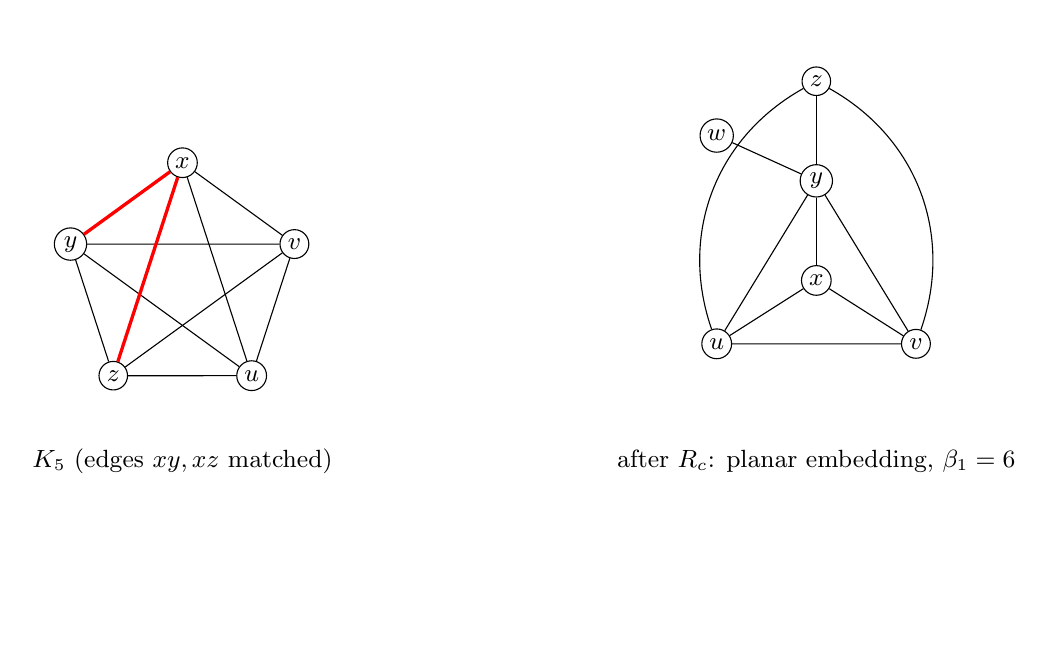
\begin{tikzpicture}[scale=1.15,every node/.style={circle,draw,fill=white,inner sep=1.5pt,font=\small}]
\begin{scope}
\foreach \i/\n in {0/x,1/y,2/z,3/u,4/v}{\node (a\n) at ({90+72*\i}:1.3) {$\n$};}
\foreach \p/\q in {x/y,x/z,x/u,x/v,y/z,y/u,y/v,z/u,z/v,u/v}{\draw (a\p)--(a\q);}
\draw[red,very thick] (ax)--(ay); \draw[red,very thick] (ax)--(az);
\node[draw=none,fill=none] at (0,-2) {$K_5$ (edges $xy,xz$ matched)};
\end{scope}
\begin{scope}[xshift=7cm]
\node (by) at (0,1.1) {$y$}; \node (bu) at (-1.1,-0.7) {$u$}; \node (bv) at (1.1,-0.7) {$v$};
\node (bx) at (0,0) {$x$}; \node (bz) at (0,2.2) {$z$}; \node (bw) at (-1.1,1.6) {$w$};
\draw (by)--(bu)--(bv)--(by);
\draw (bx)--(by); \draw (bx)--(bu); \draw (bx)--(bv);
\draw (bz) to[bend right=40] (bu); \draw (bz) to[bend left=40] (bv); \draw (bz)--(by);
\draw (by)--(bw);
\node[draw=none,fill=none] at (0,-2) {after $R_c$: planar embedding, $\Betti=6$};
\end{scope}
\end{tikzpicture}}
\caption{Proposition~\ref{prop:counter}. $R_c$ deletes $xy,xz$ and adds $xy,yz,yw$. The multigraph keeps $\Betti=6$ (the added $yz$ is parallel to an existing edge, drawn once), but the simple graph is $K_5-xz$ with a pendant vertex, which is planar. The drawing is the triangular bipyramid on $\{y,u,v\}$ with apexes $x$ and $z$.}\label{fig:counter}
\end{figure}

%==============================================================================
\section{Minor preservation implies persistence of non-planarity}
\begin{theorem}[Protection by minor preservation]\label{thm:protect}
Let $H_0\to\dots\to H_t$ be any sequence of events (any order).
\begin{enumerate}
\item[(a)] If $R$ is minor-preserving, $H_0$ is a minor of $H_t$. Hence if $H_0$ is non-planar then $H_t$ is non-planar for all $t$, and $\Betti(H_t)\ge\Betti(H_0)$.
\item[(b)] If $R$ is path-preserving, $H_t$ contains a subdivision $\sigma_t(H_0)$ of $H_0$, where $\sigma_t$ sends each subgraph $F\subseteq H_0$ to a subdivision $\sigma_t(F)\subseteq H_t$ of $F$ (so $\Betti(\sigma_t(F))=\Betti(F)$), with $\sigma_t(A\cap B)=\sigma_t(A)\cap\sigma_t(B)$ and $\sigma_t(A\cup B)=\sigma_t(A)\cup\sigma_t(B)$.
\item[(c)] If $R$ is simple-minor-preserving, the simple graph of $H_0$ is a minor of that of $H_t$; hence $H_t$ is non-planar for all $t$ whenever $H_0$ is.
\end{enumerate}
\end{theorem}
\begin{proof}
(a) One event: in $H'=(H-L_m)\cup K_m$ contract, for each old variable $a$, the connected set of vertices $\varphi(B_a)$ to the single vertex $\varphi(a)$ (possible by Definition~\ref{def:minor}(i); the other vertices of $H$ are untouched since each branch set contains exactly one old vertex). The result contains $H-L_m$ and, by (ii), an edge between $\varphi(a)$ and $\varphi(b)$ for every edge of $L_m$, so it contains $H$ as a subgraph; thus $H$ is a minor of $H'$. Minors are transitive, so $H_0$ is a minor of $H_t$. Planarity is closed under taking minors \citep{diestel2017}, and by Wagner's theorem \citep{wagner1937} is characterised by the excluded minors $K_5$ and $K_{3,3}$; so $H_t$ planar would force $H_0$ planar. For $\Betti$: contraction preserves it and passing to a subgraph does not increase it, so $\Betti(H_0)\le\Betti(H_t)$.
(c) The same contraction yields a graph that contains $H-L_m$ and, for each distinct pair $\{\varphi(a),\varphi(b)\}$ of $L_m$, an edge between them; so it contains the simple graph of $H$.
(b) One event: let $P_1,P_2$ be the paths for the two edges of $L_m$. Put $S=(H-L_m)\cup\varphi(P_1)\cup\varphi(P_2)$. Internal vertices are fresh and distinct and the paths use distinct edges of $K_m$, so $S\subseteq H'$ is $H$ with two edges subdivided. Define $\tau(F)$ as $F$ with each edge replaced by itself or its path; $\tau$ commutes with $\cap,\cup$ because edges map to pairwise disjoint edge sets and vertices to themselves. Compose: $\sigma_{s+1}=\tau_s\circ\sigma_s$; a subdivision of a subdivision of $F$ is a subdivision of $F$. Subdividing an edge adds one vertex and one edge, so preserves $\Betti$.
\end{proof}
\begin{remark}
Theorem~\ref{thm:protect} needs no closedness, confluence, lattice background or choice of defect. A large 3D lattice is itself non-planar, so global planarity is a useful witness only on planar backgrounds, and even there only until the rule itself creates non-planarity (Section~\ref{sec:exp}).
\end{remark}

\begin{proposition}[Non-injective matches]\label{prop:noninj}
Allow states with loops and parallel edges, and matches $\varphi$ that need not be injective on $\var(L)$: two distinct variables may be sent to the same vertex, and the two edges of $L$ go to two distinct edges of the state, which may be loops. Take minors in the multigraph sense (loops allowed). Then Theorem~\ref{thm:protect}(a) and~(c) hold verbatim; (b) holds if a loop may be subdivided into a cycle. Consequently Theorem~\ref{thm:dichotomy} holds unchanged for the larger event relation, and so do Theorem~\ref{thm:euler} and Corollary~\ref{cor:global} (their proofs do not use injectivity).
\end{proposition}
\begin{proof}
Let $R$ be minor-preserving with a branch assignment as in Definition~\ref{def:minor}, and let one event with match $\varphi$ turn $H$ into $H'=(H-L_m)\cup K_m$. For each old variable $a$ choose a spanning tree $T_a$ of the $K$-edges inside the connected branch set $B_a$. Since $B_a$ contains exactly one old variable, every edge of $T_a$ has at least one fresh end, so its image in $H'$ is not a loop. The fresh vertices of distinct branch sets are distinct, so the trees $T_a$ are edge-disjoint and can be contracted one after the other: each contraction merges fresh vertices into $\varphi(a)$ and nothing else. This is well defined also when $\varphi(a)=\varphi(b)$ for $a\neq b$. Then delete the fresh vertices assigned to $\bot$. The result contains $H-L_m$ (untouched), and, for every $K$-edge between two distinct branch sets $B_a,B_b$, an edge from $\varphi(a)$ to $\varphi(b)$, which is a loop if $\varphi(a)=\varphi(b)$. By Definition~\ref{def:minor}(ii) these include a copy of $\varphi(e)$ for every edge $e$ of $L$, loops included, so the result contains $H$ as a sub-multigraph and $H$ is a minor of $H'$. Transitivity along the sequence gives (a). Loops do not affect planarity, and a minor of multigraphs induces a minor of simple graphs; this gives the planarity statement of (a). For (c), a distinct pair $\{a,b\}$ of $L$ is joined by an inter-branch edge, which gives $\varphi(a)\varphi(b)$, an edge of the simple graph of $H$ unless it is a loop. For (b), in the argument of Theorem~\ref{thm:protect}(b) the path for an edge $(a,b)$ with $\varphi(a)=\varphi(b)$ becomes a closed path through fresh vertices, a subdivided loop. For the final claim: (i)$\Rightarrow$(ii) of Theorem~\ref{thm:dichotomy} now holds for all events by (c), and (ii)$\Rightarrow$(iii) is trivial because injective matches are matches.
\end{proof}
\noindent\emph{Where injectivity does matter.} The usual picture, in which $H$ is obtained by contracting the \emph{disjoint} branch sets $\varphi(B_a)$, is not available when $\varphi(a)=\varphi(b)$, since the two sets then share a vertex; the proof above avoids it by contracting only fresh vertices into their own old vertex. We have not checked whether the proofs of the rigidity results (Theorem~\ref{thm:rigid}, Propositions~\ref{prop:transport} and~\ref{prop:add}) survive non-injective matches, and do not claim it. As a check of the proof step, for all minor-preserving and simple-minor-preserving rules of $\mathcal S$ we applied \nimEvents{} events on $K_5$, $K_{3,3}$ and the double self-loop with tight edge multiplicities and loops at every vertex, of which \nimNonInj{} were non-injective, carried out the contraction above with the rule's branch assignment, and found $H$ in the result every time. As a negative control, none of \nimCtrl{} rules that are not simple-minor-preserving passes the same test for any valid branch assignment (\texttt{scripts/check\_noninjective\_minor.py}).

%==============================================================================
\section{Rigidity inside the minor-preserving class}\label{sec:rigid}
\begin{theorem}[Rigidity of cycle-rank-conserving minor-preserving rules]\label{thm:rigid}
Let $R$ be closed and minor-preserving with $\delta_R=0$. Fix a branch assignment as in Definition~\ref{def:minor} and an event with match $\varphi$ producing $H'$ from $H$. Then
\begin{enumerate}
\item[(i)] $H'$ is obtained from $H$ by (1) replacing each vertex $\varphi(a)$ by a tree on $\varphi(B_a)$ (a vertex expansion, the edges of $H$ not consumed remaining attached at $\varphi(a)$), re-attaching the image of each consumed edge of $L$ to vertices of these trees, and (2) attaching pendant trees, each to the rest by exactly one edge;
\item[(ii)] $H'$ is homotopy equivalent to $H$; consequently, for every sequence of events, $H_t\simeq H_0$, so $\Betti(H_t)=\Betti(H_0)$ and $c(H_t)=c(H_0)$;
\item[(iii)] if moreover $R$ is path-preserving and $H_0$ connected, then $H_t=\sigma_t(H_0)\cup F_t$ with $F_t$ a union of pendant trees (each attached by one edge), and the 2-core of $H_t$ is a subdivision of the 2-core of $H_0$.
\end{enumerate}
\end{theorem}
\begin{proof}
Let $A$ be the number of new variables assigned to old variables and $D$ the number of discarded ones, so $A+D=n_{\rm new}$. Since $K$ is loop-free, each edge of $K$ lies in exactly one of: $C$ (both ends in the same branch set $B_a$), $X$ (at least one end discarded), $M$ (ends in two distinct branch sets). So $|K|=|C|+|X|+|M|$.

\emph{Three lower bounds.} (1) $|C|\ge A$: each $B_a$ is connected by $C$-edges, so contains at least $|B_a|-1$ of them, and $\sum_a(|B_a|-1)=A$. (2) $|M|\ge|L|$: by (ii) of Definition~\ref{def:minor} the edges of $M$ cover the $|L|$ edges of $L$ as a multiset. (3) $|X|\ge D$: form the graph $Q$ whose vertices are the $D$ discarded variables and one extra vertex $s$, with one edge for every edge of $X$, in which an endpoint belonging to a branch set is replaced by $s$ ($Q$ has no loops since every $X$-edge has a discarded endpoint). Every discarded vertex $d$ is joined to $s$ in $Q$: since $K$ is connected there is a path in $K$ from $d$ to an old variable; the initial segment up to the first non-discarded vertex consists of $X$-edges and gives a path from $d$ to $s$ in $Q$. So $Q$ is connected on $D+1$ vertices and has at least $D$ edges.

\emph{Equality.} $\delta_R=0$ means $|K|=|L|+n_{\rm new}=|L|+A+D$, and (1)--(3) give $|K|\ge A+|L|+D$. Hence all three bounds are equalities. Consequently: (1$'$) the $C$-edges inside each $B_a$ form a spanning tree $T_a$ of $B_a$ (exactly $|B_a|-1$ edges that connect it), and there are no other $C$-edges, in particular no edge parallel to a tree edge; (2$'$) $M$ consists of exactly $|L|$ edges, which therefore correspond bijectively to the edges of $L$; (3$'$) $Q$ is connected with $D+1$ vertices and $D$ edges, hence a tree.

\emph{Structure.} In $H'$ contract each tree $\varphi(T_a)$ to the vertex $\varphi(a)$ and call the result $H''$. No loops arise: no extra $C$-edges exist by (1$'$), and $M$-edges join distinct branch sets. The edges of $H-L_m$ are unchanged, and by (2$'$) the $M$-edges become exactly copies of the consumed edges $L_m$ (with the same endpoints $\varphi(a),\varphi(b)$), so $H''$ contains $H$. The remaining edges are the images of $X$. By (3$'$), each component of the graph induced by the discarded vertices is a tree and is joined to $s$ (that is, to the old part) by exactly one edge of $X$; since discarded vertices are fresh and meet only $X$-edges, these are pendant trees in $H''$, each attached at one vertex $\varphi(a)$ by exactly one edge. So $H''=H\,\cup$ pendant trees, and $H'$ is obtained from $H''$ by expanding the vertices $\varphi(a)$ into the trees $\varphi(T_a)$. This is (i).

\emph{Homotopy.} Contracting a tree (a connected acyclic subgraph) in a graph is a homotopy equivalence \citep[Prop.~0.17]{hatcher2002}, as is deleting a pendant tree. Hence $H'\simeq H''\simeq H$, and composing over events gives $H_t\simeq H_0$; $\Betti$ and the number of components are homotopy invariants. This is (ii).

(iii) By Theorem~\ref{thm:protect}(b), $S=\sigma_t(H_0)\subseteq G:=H_t$ is connected, and $\Betti(S)=\Betti(H_0)=\Betti(G)$ by (ii). Contract $S$ to a vertex $s$: $G/S$ is connected with $|E|-|E_S|$ edges and $|V|-|V_S|+1$ vertices, so $\Betti(G/S)=\Betti(G)-\Betti(S)=0$ and $G/S$ is a tree. An edge of $G\setminus S$ with both ends in $S$ would be a loop at $s$, so there is none; each component of $(G/S)-s$ is joined to $s$ by exactly one edge. So $G\setminus S$ is a union of pendant trees; pruning them leaves the 2-core of $S$.
\end{proof}

\paragraph{Transported subgraphs.} Fix, for a minor-preserving rule, one branch assignment and a bijection between the edges of $L$ and $|L|$ edges of $M$ (the \emph{images}), and, among the edges of $C$, a spanning forest $T_a$ of each $B_a$. For a subgraph $D\subseteq H$ (a set of labelled edges) the \emph{transported} subgraph $D'\subseteq H'$ after an event with match $\varphi$ consists of: the edges of $D$ not consumed; the image of each consumed edge of $L$ that lies in $D$; and the trees $\varphi(T_a)$ for all $a$ with $\varphi(a)$ a vertex of $D$ (vertices are taken before the event). For a generation step the same definition is applied to all its events using the vertex set of $D$ before the step. Several subgraphs $D_1,D_2$ are transported independently.

\begin{proposition}[Transported subgraphs]\label{prop:transport}
Let $R$ be minor-preserving (any $\delta_R$), $D_1,D_2\subseteq H_0$ subgraphs, and $D_i(t)$ their transports along any sequence of events or generation steps. Then for all $t$: (a) $D_i(t)\simeq D_i(0)$, so $\Betti(D_i(t))=\Betti(D_i(0))$; (b) $D_i(0)$ is a minor of $D_i(t)$, so $D_i(t)$ is non-planar if $D_i(0)$ is; (c) $D_1(t)\cup D_2(t)\simeq D_1(0)\cup D_2(0)$, so $\iota(D_1(t),D_2(t))=\iota(D_1(0),D_2(0))$ and $\Betti(D_1(t)\cup D_2(t))-\Betti(D_1(t))-\Betti(D_2(t))$ is constant.
\end{proposition}
\begin{proof}
Consider one generation step. Contract in $H'$ every transported tree $\varphi(T_a)$ to its root $\varphi(a)$. Trees of different events meet only at a common root (their non-root vertices are fresh), so the contraction is well defined, and the contracted subgraph is: the unconsumed edges of $D$, and, for each consumed labelled edge, its image with ends moved to $\varphi(a),\varphi(b)$, that is, the consumed edge itself. So the contraction of $D'$ is exactly $D$. Contracting a forest is a homotopy equivalence, and it exhibits $D$ as a minor of $D'$; this proves (a) and (b) for one step, and composition proves them for all $t$. For (c) let $\pi:H'\to H''$ be the contraction of all transported trees (the same map for both subgraphs). A tree rooted at $v$ lies in $D_i'$ exactly when $v$ is a vertex of $D_i$ (its edges carry the labels of the edges at $v$), hence in $D_1'\cap D_2'$ exactly when $v$ is a vertex of both. Therefore $\pi$ maps $D_1'$, $D_2'$, $D_1'\cap D_2'$ and $D_1'\cup D_2'$ onto $D_1$, $D_2$, $D_1\cap D_2$ and $D_1\cup D_2$ respectively, in each case by contracting a forest, which preserves the number of components and $\Betti$. By Lemma~\ref{lem:mv}, $\iota$ is a function of exactly these eight numbers, so it is unchanged by the step; induction on steps finishes the proof.
\end{proof}

\begin{corollary}[Trade-off inside the minor-preserving class]\label{cor:tradeoff}
Let $R$ be closed and minor-preserving, $H_0$ non-planar. For every sequence of $N$ events: non-planarity persists; and either (a) $\delta_R=0$, then $\Betti(H_N)=\Betti(H_0)$ and $H_N\simeq H_0$; or (b) $\delta_R>0$, then $\Betti(H_N)=\Betti(H_0)+N\delta_R$ is unbounded. In both cases each transported defect keeps its cycle rank and two transported defects keep their interaction term.
\end{corollary}
\noindent The statement is therefore \emph{not} that protection and conservation of a defect's cycle rank exclude each other: with transport, a defect's cycle rank is conserved for all minor-preserving rules. What the class loses for $\delta_R>0$ is conservation of the \emph{global} cycle rank, and what it has for $\delta_R=0$ is a frozen homotopy type of the whole graph. In either case cycle rank cannot be exchanged between transported defects. Whether other, non-transported notions of a defect (for instance a geometric neighbourhood) can interact non-trivially is not addressed.

%==============================================================================
\section{An exhaustive classification}\label{sec:class}
Let $\mathcal S$ be the set of closed loop-free rules of signature $2_2\to3_2$ with $n_{\rm new}\le1$ or $2_2\to4_2$ with $n_{\rm new}\le2$, up to renaming of variables and edge order ($|\mathcal S|=5225$: 424 and 4801).
\begin{theorem}[Dichotomy on $\mathcal S$; computer-assisted]\label{thm:dichotomy}
For $R\in\mathcal S$ the following are equivalent: (i) $R$ is simple-minor-preserving; (ii) for every non-planar $H_0$ and every sequence of events, every $H_t$ is non-planar; (iii) no single event applied to the simple $K_5$ (edges directed from lower to higher index) yields a graph with planar underlying simple graph.
\end{theorem}
\begin{proof}
(i)$\Rightarrow$(ii) is Theorem~\ref{thm:protect}(c); (ii)$\Rightarrow$(iii) is trivial. For (iii)$\Rightarrow$(i), in contrapositive, we need, for every rule of $\mathcal S$ that is not simple-minor-preserving, one event on \emph{the host named in (iii)}, namely $K_5$ with every edge $(a,b)$, $a<b$, directed from lower to higher index (``$A_5$''), whose output has a planar simple projection. The search program tried four hosts in a fixed order ($A_5$, the analogous $K_{3,3}$, and two versions with doubled edges) and stopped at the first planarising event; \emph{all 2388 certificates were found on $A_5$, the first host}, so the statement (iii) is certified exactly as written and the other hosts played no role in the proof. A certificate records the rule, the match, the output edge list and a rotation system. The standalone checker \texttt{verify\_certificates.py} (Python standard library only, sharing no code with the search) establishes: (1) every certificate has host $A_5$; (2) re-applying the recorded event to $A_5$ reproduces the recorded output; (3) the rotation system is a valid planar embedding of the output's simple projection (faces traced and Euler's formula $n-m+f=1+c$ checked); (4) with its own brute-force decision procedure the checker finds exactly 2388 of the 5225 rules in the rule list to be not simple-minor-preserving, and the set of certified rules equals this set, each rule certified once; (5) no simple-minor-preserving rule has a certificate. All checks pass (log in Appendix~\ref{app:audit}). The proof is exhaustive but computer-assisted: besides the certificates it relies on the rule list being complete, which was cross-checked by a Burnside count (Appendix~\ref{app:audit}), and on the checker's decision procedure, which is also implemented independently of the main code.
\end{proof}

\begin{lemma}[$Y\to\Delta$ preserves planarity]\label{lem:YDelta}
Let $G$ be planar with a vertex $w$ of degree $3$ whose neighbours $x,y,z$ are distinct. Deleting $w$ and adding the edges $xy,yz,zx$ gives a planar graph.
\end{lemma}
\begin{proof}
In a planar embedding the edges $wx,wy,wz$ leave $w$ in some cyclic order. Delete $w$ and draw $xy,yz,zx$ along the former edges in a small neighbourhood of $w$; each new arc follows two former edges that are adjacent in the rotation at $w$, so it crosses neither the other arcs nor the rest of the drawing.
\end{proof}

\begin{proposition}[Necessity fails in general signatures]\label{prop:necfail}
(a) ($\Delta\to Y$) The rule $\{\{1,2\},\{1,3\},\{2,3\}\}\to\{\{1,4\},\{2,4\},\{3,4\}\}$ (signature $3_2\to3_2$) is closed and not simple-minor-preserving, but whenever $H$ is non-planar the output of every event is non-planar. It does not preserve planarity.
(b) (Kuratowski gadget) Let $L=\{\{1,2\},\{1,3\}\}$ and $K=\{\{1,2\},\{2,4\},\{3,4\}\}\cup\{\{a,b\}:a\in\{4,5,6\},\,b\in\{7,8,9\}\}$ (signature $2_2\to12_2$). The rule is closed and not simple-minor-preserving, but every event produces a non-planar graph, whatever the host.
\end{proposition}
\begin{proof}
(a) The new vertex $w$ of the output $H'$ has degree exactly $3$ (its edges are the three edges of $K$), with distinct neighbours $x,y,z$ the images of $1,2,3$. Deleting $w$ and adding the triangle $xy,yz,zx$ gives a graph whose underlying simple graph is that of $H$ (the event removed one copy of each triangle edge). By Lemma~\ref{lem:YDelta}, $H'$ planar would imply $H$ planar; so $H$ non-planar implies $H'$ non-planar. Not simple-minor-preserving: the left side has the three distinct pairs $\{1,2\},\{1,3\},\{2,3\}$ and the only new variable is $4$; $K$ is a star centred at $4$, so whichever branch set absorbs $4$ (or if it is discarded), at most two of the three pairs are joined between their branch sets. Planarity is not preserved: it is not claimed from the proof but observed (480 events on random planar hosts gave non-planar graphs, Appendix~\ref{app:audit}); a planar host with a separating triangle gives an example, since three bridges attached at $x,y,z$ then form a $K_{3,3}$ minor.
(b) The output contains $K\supseteq K_{3,3}$ (on new vertices), hence is non-planar. Not simple-minor-preserving: variable $1$ has the single neighbour $2$ in $K$, which is old, so $B_1=\{1\}$ and its only neighbouring branch set is $B_2$; the pair $\{1,3\}$ is not covered.
\end{proof}
\noindent So minor preservation is not the only protection mechanism: $Y\!\to\!\Delta$ equivalence is another, and a right side containing a Kuratowski graph is a trivial third (which requires at least $9$ edges on the right).

\paragraph{Why no $\Delta\to Y$-type exception occurs in $\mathcal S$ (explanation, not a proof).} In Proposition~\ref{prop:necfail}(a) the closing side $\{2,3\}$ of the triangle is covered by no branch-set edge, yet planarity cannot see the loss, because Lemma~\ref{lem:YDelta} trades the degree-3 vertex for the triangle. The mechanism needs the simple graph of $L$ to contain a cycle, so that an adjacency removed by the event can be restored by a planar duality. For $R\in\mathcal S$ the left side has two edges. As a multigraph it can contain a cycle (a digon, if the two edges are parallel or antiparallel), but its simple graph is always a forest: a single pair, or a path on three vertices. So every pair of $L$ that the rule fails to cover is an adjacency that is really destroyed, and there is no third adjacency for a duality to recover. What this does \emph{not} explain is why destroying an adjacency always lets an event on $K_5$ end in a planar graph for all $2388$ rules; that is what the certificates show, and we have no conceptual proof of it. The bounded search of Section~\ref{sec:general} agrees with the explanation: for $m=2$ and $k=3,\dots,7$ no exception occurs, and the exceptions begin at $m=3$, where $L$ can be a triangle. Necessity for all $2$-edge left sides, without a bound on $k$, is open.

\subsection{A bounded search beyond $\mathcal S$ (evidence, not a proof)}\label{sec:general}
To see how far (iii)$\Rightarrow$(i) extends, \texttt{general\_signature\_search.py} repeats the certificate search for further signatures $m_2\to k_2$, with a generalised enumerator that reproduces $\mathcal S$ exactly. Hosts are $K_5$ and $K_{3,3}$ with the left side planted with its exact multiplicities (all injective placements of the old variables), plus the simple and doubled versions. Table~\ref{tab:general} gives the outcome. Rules that are simple-minor-preserving never planarised a host in the sampled matches (0 planarisations, as Theorem~\ref{thm:protect} requires). For $m=1$ every closed rule is simple-minor-preserving. For $m=2$ and $k=3,\dots,7$ every rule that is not simple-minor-preserving has a certificate: necessity held for all rules searched. The exceptions occur only for $m=3$, and are exactly the $\Delta\to Y$ variants of Proposition~\ref{prop:necfail}(a) (no unexplained case). The search is bounded: the bounds on new variables are not exhaustive for $k\ge5$, the $m=3$ signatures were searched with at most one new variable, and a rule without a certificate on the hosts used is only a candidate counterexample (each was explained here).
\begin{table*}[t]\centering\scriptsize
\resizebox{\textwidth}{!}{\begin{tabular}{lrrrrrr}
\toprule
signature $m_2\to k_2$ ($n_{\rm new}\le$) & closed rules & simple-minor-pres. & not s.m., certificate & not s.m., no certificate: $\Delta\!\to\!Y$ & Kuratowski gadget & unexplained\\
\midrule
$1_2\to2_2$ (1) & 15 & 15 & 0 & 0 & 0 & 0\\
$1_2\to3_2$ (2) & 116 & 116 & 0 & 0 & 0 & 0\\
$1_2\to4_2$ (2) & 532 & 532 & 0 & 0 & 0 & 0\\
$1_2\to5_2$ (3) & 5238 & 5238 & 0 & 0 & 0 & 0\\
$3_2\to3_2$ (1) & 2060 & 568 & 1480 & 12 & 0 & 0\\
$3_2\to4_2$ (1) & 22230 & 4546 & 17636 & 48 & 0 & 0\\
$2_2\to5_2$ (3) & 49622 & 28510 & 21112 & 0 & 0 & 0\\
$2_2\to6_2$ (2) & 141296 & 88104 & 53192 & 0 & 0 & 0\\
$2_2\to7_2$ (1) & 59632 & 42480 & 17152 & 0 & 0 & 0\\
\bottomrule
\end{tabular}
}
\caption{\textbf{Bounded} necessity search beyond $\mathcal S$ (closed loop-free rules up to renaming); the bound on new variables $n_{\rm new}$ is shown for each signature and is not exhaustive for $k\ge5$. A rule with a certificate is proved to violate protection on one host; the table makes no claim about rules outside these bounds, and ``no certificate'' is only a candidate counterexample. ``Not s.m., no certificate'' is split by the explanation found.}\label{tab:general}
\end{table*}

\subsection{Planarity-preserving rules and their overlap with minor preservation}\label{sec:planarity}
The tangle heuristic of \citet[\S2.4]{gorard2020relativistic} needs two things: tangles persist, and the planar background stays planar. Theorem~\ref{thm:dichotomy} settles the first for $\mathcal S$. For the second, call $R$ \emph{planarity-preserving} if for every state whose simple graph is planar and every event the output has a planar simple graph. For a rule $R=(L\to K)$ write $G$ for the simple graph of $K$ on $\var(K)$, $O=\var(L)$ for the old and $N$ for the new variables, and $\mathrm{pairs}(L)$ for the distinct unordered pairs of vertices joined by an edge of $L$. Say that $R$ satisfies condition $P$ if
\begin{enumerate}
\item[(P1)] every edge of $G$ between two old variables is a pair of $\mathrm{pairs}(L)$;
\item[(P2)] every connected component $C$ of $G[N]$ has at most two old neighbours; if it has two, $\{a,b\}$, then $\{a,b\}\in\mathrm{pairs}(L)$ and $G[C\cup\{a,b\}]+ab$ is planar.
\end{enumerate}
In words: apart from edges that $L$ already had, $K$ may add only pendant pieces and ``ears'' between the two ends of an edge of $L$; it may not join two old vertices that $L$ did not join, and no new vertex may see three old vertices (that is a vertex split, as in the star rule).

\begin{lemma}[Substitution]\label{lem:subst}
Let $G'$ be planar, $uv$ an edge of $G'$, and $B$ a graph with $V(B)\cap V(G')=\{u,v\}$ such that $B+uv$ is planar. Then $G'\cup B$ is planar. If $B$ meets $G'$ in a single vertex and both are planar, $G'\cup B$ is planar.
\end{lemma}
\begin{proof}
Embed $B+uv$ with the edge $uv$ on the outer face and shrink it into a thin neighbourhood of the edge $uv$ of an embedding of $G'$; the edge $uv$ of $B+uv$ is then identified with $uv$. For one common vertex, place $B$ inside a face at that vertex.
\end{proof}

\begin{proposition}[$P$ implies planarity preservation]\label{prop:Pplanar}
If $R$ satisfies $P$, then for every state with planar simple graph and every event, injective or not, the output has a planar simple graph. Every closed rule of $\mathcal S$ satisfying $P$ is simple-minor-preserving.
\end{proposition}
\begin{proof}
Let $H$ be planar and $H'=(H-L_m)\cup K_m$. The old-old edges of $K_m$ join images of pairs of $\mathrm{pairs}(L)$, which are edges of the simple graph of $H$ (or loops, which do not count). Each component $C$ of fresh vertices with old neighbours $A$ is attached to $\varphi(A)$ only. If $|A|=1$, or $|A|=2$ with $\varphi(a)=\varphi(b)$, it meets the rest in one vertex. If $|A|=2$ with $\varphi(a)\neq\varphi(b)$, then $\varphi(a)\varphi(b)$ is an edge of $H$ and the piece $B=G[C\cup A]$ satisfies $B+ab$ planar by (P2). Add the pieces one at a time using Lemma~\ref{lem:subst} (the edge $\varphi(a)\varphi(b)$ stays in the graph, so several ears on one edge are fine). The simple graph of $H'$ is a subgraph of the result, hence planar.
For the second claim let $R\in\mathcal S$ satisfy $P$. The simple graph of $L$ has at most two edges and is connected on $O$, so it is a tree. Let $\Gamma$ be the graph on $O$ with an edge $ab$ whenever $ab\in G$ or some component $C$ has old neighbours exactly $a,b$. By (P1),(P2) all edges of $\Gamma$ are pairs of $L$, and since $K$ is connected (pendant components do not connect anything) $\Gamma$ is connected; a connected spanning subgraph of a tree is the tree, so every pair of $L$ is an edge of $G$ or has an ear. Assign each fresh vertex of a component to one of its old neighbours (a component with two old neighbours to either one). Branch sets are connected, since each component is adjacent to the old variable it is assigned to, and each pair of $L$ is joined by an edge between its branch sets. So $R$ is simple-minor-preserving.
\end{proof}

\begin{theorem}[Planarity-preserving rules on $\mathcal S$; computer-assisted]\label{thm:planarity}
For $R\in\mathcal S$ the following are equivalent: (i) $R$ satisfies $P$; (ii) $R$ is planarity-preserving; (iii) no event, with a planar host taken from the six graphs below, has a non-planar output.
\end{theorem}
\begin{proof}
(i)$\Rightarrow$(ii) is Proposition~\ref{prop:Pplanar}; (ii)$\Rightarrow$(iii) is trivial. For (iii)$\Rightarrow$(i) we need, for each of the $\plnNonP$ rules of $\mathcal S$ that violate $P$, a planar host and a match with non-planar output. The script \texttt{scripts/planarity\_preserving.py} searches hosts built from the octahedron, cube, icosahedron, $K_4$, the wheel with five spokes and the $3\times3$ grid: an injective placement of the old variables, the pairs of $L$ added if absent (kept only if the result is planar), every edge present in four copies (both orientations twice) so that every pattern matches. The output's simple graph is the host plus the image of $K$ with fresh new vertices. All $\plnNonP$ rules violating $P$ have such a certificate, every one found on the first base, the octahedron. No rule satisfying $P$ has a non-planar output on any placement and host, as Proposition~\ref{prop:Pplanar} requires. The decision of $P$ and the search are separate computations over the same enumeration as Theorem~\ref{thm:dichotomy}; they were not re-implemented independently, so this half of the statement rests on one implementation, and certificates are listed in \texttt{results/planarity/planarity\_classification.csv}.
\end{proof}

\begin{table*}[t]\centering\scriptsize
\begin{tabular}{lrrrrrr}
\toprule
signature & rules & simple-minor-pres. & planarity-pres. ($P$) & $P$, $\delta_R=0$ & $P$, $\delta_R>0$ & s.m.-pres., not planarity-pres.\\
\midrule
$2_2\to3_2$ & 424 & 216 & 180 & 150 & 30 & 36\\
$2_2\to4_2$ & 4801 & 2621 & 1929 & 1269 & 660 & 692\\
\midrule
all of $\mathcal S$ & 5225 & 2837 & 2109 & 1419 & 690 & 728\\
\bottomrule
\end{tabular}

\caption{Planarity preservation within $\mathcal S$ (Theorem~\ref{thm:planarity}). Every planarity-preserving rule is simple-minor-preserving (Proposition~\ref{prop:Pplanar}); the last column counts the simple-minor-preserving rules that nevertheless fail to preserve planarity.}\label{tab:planarity}
\end{table*}

Table~\ref{tab:planarity} gives the overlap. Of the $\plnAll$ rules, $\plnNotSM$ do not even protect non-planarity, $\plnSMnotP$ protect it but do not preserve planarity, and $\plnP$ ($40\%$ of $\mathcal S$, $74\%$ of the minor-preserving rules) do both; $\plnPzero$ of those have $\delta_R=0$ and $\plnPgrow$ have $\delta_R>0$. So within $\mathcal S$ the intersection that the heuristic needs is not small, but it excludes natural rules. The star rule $\{\{1,2\},\{1,3\}\}\to\{\{1,4\},\{2,4\},\{3,4\}\}$ (F3 in Appendix~\ref{app:exp}) is minor-preserving yet splits a vertex: on the octahedron, with $2,3$ opposite around $1$, the output is non-planar. The triangle-closing rules G1 and G2 add an adjacency $\{2,3\}$ that $L$ did not have.

This agrees with the control runs of Appendix~\ref{app:exp}: of the 13 selected rules, F1, F2, F4 and G3 satisfy $P$ and the planar grid never became non-planar under them; G1 and G2 violate $P$ and the grid became non-planar at generation~2. F3 violates $P$ but the grid stayed planar in those runs, which is no contradiction, since a certificate needs a host in which the split edges are not consecutive around the vertex and the grid does not provide one at that scale. The proposition and the table concern the simple graph and binary rules; nothing is claimed for hyperedges.

%==============================================================================
\section{Two defects: additivity of cycle rank}\label{sec:two}
\begin{lemma}[Inclusion--exclusion for cycle rank]\label{lem:mv}
Let $A,B$ be subgraphs of a graph, $U=A\cup B$, $I=A\cap B$ (shared vertices and edges). Then $\Betti(U)=\Betti(A)+\Betti(B)+\iota(A,B)$ with $\iota(A,B)=c(I)-\Betti(I)+c(U)-c(A)-c(B)$.
\end{lemma}
\begin{proof}
$|E_U|=|E_A|+|E_B|-|E_I|$ and likewise for vertices; writing $\Betti-c=|E|-|V|$ gives $\Betti(U)-c(U)=\Betti(A)-c(A)+\Betti(B)-c(B)-\Betti(I)+c(I)$.
\end{proof}
\begin{proposition}[Non-additivity of overlapping defects]\label{prop:add}
$\Betti(D_1\cup D_2)=\Betti(D_1)+\Betti(D_2)$ iff $\iota(D_1,D_2)=0$. This holds for vertex-disjoint subgraphs and for connected subgraphs meeting in a nonempty tree. It fails for connected subgraphs meeting in a connected subgraph with a cycle ($\iota=-\Betti(I)<0$; two copies of $K_5$ sharing a triangle: $6+6$ but $\Betti(U)=11$) and for connected subgraphs meeting in $k\ge2$ tree components ($\iota=k-1>0$). For transported subgraphs of a minor-preserving rule, $\iota$ is constant (Proposition~\ref{prop:transport}).
\end{proposition}
\begin{proof}
The criterion is Lemma~\ref{lem:mv}. Disjoint: $I=\emptyset$, $c(I)=\Betti(I)=0$, $c(U)=c(A)+c(B)$. Connected $A,B$ and connected nonempty $I$: $\iota=1-\Betti(I)+1-2=-\Betti(I)$. $k$ tree components: $\iota=k+1-2=k-1$. Triangle example: $|V|=7$, $|E|=17$, $\Betti=17-7+1=11$.
\end{proof}
\noindent Since $\Betti$ is unsigned, an ``opposite orientation'' of two subgraphs has no meaning here; a signed charge would need an orientation of $H_1$ (for instance homology of a chosen embedding), not defined in this paper.

%==============================================================================
\section{Experiments}\label{sec:exp}
The theorems above are mathematical; the experiments answer two specific questions.
\begin{description}
\item[Q1 (consistency).] Do lattice evolutions with embedded defects agree with the predictions of Corollary~\ref{cor:global} and Theorems~\ref{thm:protect}--\ref{thm:rigid}, class by class? These runs are consistency checks of statements already proved, not independent evidence.
\item[Q2 (tracking).] Does the naive \emph{causal-cone labelling} of a defect, in which every product edge of an event inherits the labels of the consumed edges, define a conserved cycle-rank charge, as opposed to the minor-model transport of Proposition~\ref{prop:transport}?
\end{description}
\paragraph{Set-up.} The rules are the 126 closed $2_2\to3_2$ rules that pass a bounded joinability filter and match a simple host (88 with $\delta_R=0$ and minor-preserving, 18 with $\delta_R>0$ and minor-preserving, 20 not simple-minor-preserving; the 18 joinable rules that never match a simple host are excluded). The filter (details in Appendix~\ref{app:exp}) tests joinability of single-event divergences on finitely many small states; it is a necessary-condition filter, not a proof of confluence, and is used only to select rules. For each rule: a planar $8\times8$ grid and $3$D grids of sizes $4$ and $7$; a $K_5$ or $K_{3,3}$ embedded on grid vertices (a single defect, or two at separation $3$); canonical and seeded random update orders; $t\le10$ generations, aborting when $|E|>15000$ (some $7\times7\times7$ runs stop earlier). Defects are tracked either by cone labelling or, for minor-preserving rules, by transport. Code, seeds and data are in the archive (Appendix~\ref{app:audit}).

\paragraph{Q1: cycle-rank law and persistence.} 6032 of 6032 evolutions (all rules, both tracking modes, all backgrounds) satisfy $\Betti(H_t)=\Betti(H_0)+\delta_R\cdot(\text{events up to }t)$ at every step, as Corollary~\ref{cor:global} requires; the 13 selected rules of Appendix~\ref{app:exp} add 520 of 520 evolutions, also with no violation. On the 2D grid the cone-labelled defect stays non-planar for all $t\le10$ for all 106 minor-preserving rules and for none of the 20 other rules (Table~\ref{tab:joinable}), in line with Theorem~\ref{thm:protect} and Theorem~\ref{thm:dichotomy}. Global planarity of the 2D background is not a reliable witness: without any defect the planar grid becomes non-planar by itself under most of the rules (Appendix~\ref{app:exp}).

\paragraph{Q2: tracking.} With cone labelling the sum $\Sigma=\Betti(D_1)+\Betti(D_2)$ is conserved in all four 2D collision runs for only 48 of the 88 $\delta_R=0$ rules and 6 of the 18 $\delta_R>0$ rules, and for none of the 20 non-minor-preserving rules; $\Sigma$ grows (to thousands for $\delta_R>0$) because events that consume a defect edge and a background edge label all their product edges, so the labelled subgraph absorbs background cycles (Figure~\ref{fig:coll}, left). With minor-model transport, $\Sigma$ is conserved and $\iota_t\equiv0$ for all 106 minor-preserving rules (Figure~\ref{fig:coll}, right), as Proposition~\ref{prop:transport} proves. Hence causal-cone labelling is not a valid definition of a conserved defect charge, even for rules where protection is a theorem.
\begin{table*}[t]\centering\scriptsize
\begin{tabular}{lrcccc}
\toprule
class & rules & $D$ non-planar $\forall t$ (2D, cone) & $\Sigma$ conserved (cone) & $\Sigma$ conserved (model) & $\iota_t\equiv0$ (model)\\
\midrule
protected\_frozen & 88 & 88/88 & 48/88 & 88/88 & 88/88\\
protected\_cycle\_growing & 18 & 18/18 & 6/18 & 18/18 & 18/18\\
dissolving & 20 & 0/20 & 0/20 & -- & --\\
\bottomrule
\end{tabular}

\caption{All 126 joinable $2_2\to3_2$ rules, 2D grid ($n=8$), $K_5$ and $K_{3,3}$, canonical and random order (4 runs per rule and experiment). Entries: rules for which the property holds in all 4 runs / rules with complete data. ``Cone'': causal-cone labelling; ``model'': minor-model transport.}\label{tab:joinable}
\end{table*}
\begin{figure*}[t]\centering
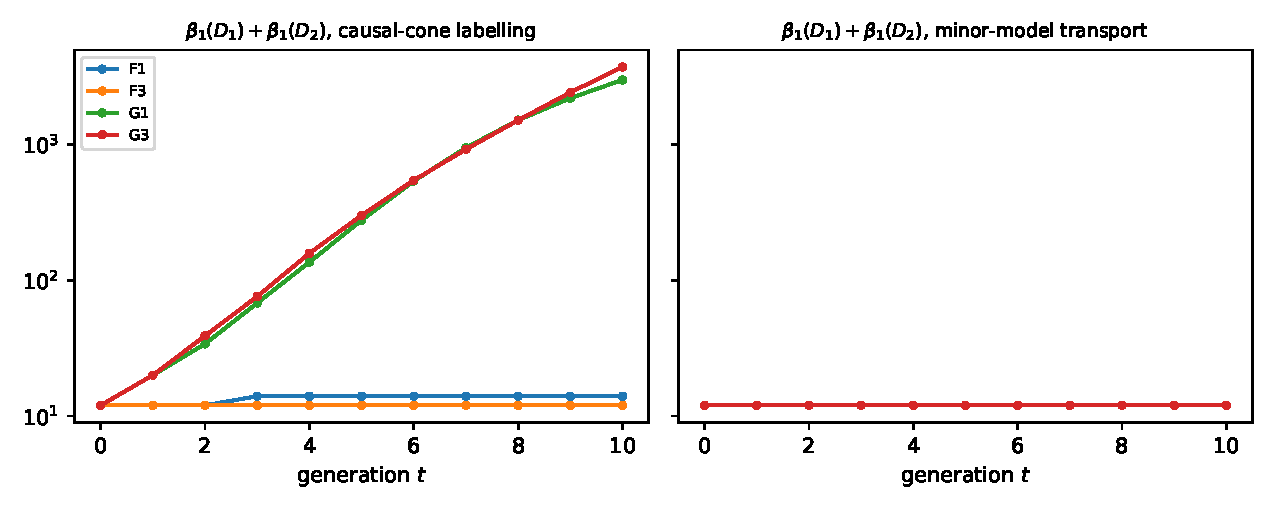
\includegraphics[width=0.85\textwidth]{figs/fig_collision.pdf}
\caption{$\beta_1(D_1)+\beta_1(D_2)$ along $K_5$ collisions on the 2D grid (canonical order, four selected rules): cone labelling (left, symlog axis) and minor-model transport (right).}\label{fig:coll}
\end{figure*}
\paragraph{Limitations of the experiments.} The horizon is $t\le10$ generations (the edge cap stops some runs earlier); rules are those passing a bounded filter; backgrounds are small; no claim about continuum limits or particle behaviour is made (additional descriptive measurements are in the archive).

%==============================================================================
\section{Relation to the Wolfram model}\label{sec:wolfram}
This section states how the rewriting systems studied here relate to those of the Wolfram Physics Project, which claim is being tested, and how far the results reach. The model is that of \citet{wolfram2020class}; the discussion of oligons and non-planar tangles is in \citet{wolfram2020project,wolframtechintro} and \citet[\S2.4]{gorard2020relativistic}.

\subsection{What the class studied here is}
\emph{Setting in the Wolfram model.} A state is a hypergraph, a collection of ordered relations of arbitrary arity; a rule replaces a sub-hypergraph matching a pattern by another; a rule's \emph{signature} counts the relations of each arity on each side, written $n_k$ for $n$ relations of arity $k$, so ``$2_2\to4_2$'' is two binary relations replaced by four \citep{wolframtechrules}; the Technical Background also treats rules of mixed arity. The standard initial condition in the papers we looked at is a pair of self-loops, $\{\{0,0\},\{0,0\}\}$, and an evolution proceeds in generations in which a maximal set of non-overlapping matches is applied. Evolution is non-deterministic in general, since there is no canonical update order.

\emph{Our class.} The rules studied are those of \emph{pure arity two}: signatures $n_2\to m_2$, mostly with $n=2$ (Theorem~\ref{thm:dichotomy} covers $2_2\to3_2$ and $2_2\to4_2$ exhaustively; Section~\ref{sec:general} searches further signatures with $n=1,2,3$). For such rules the spatial hypergraph is an ordinary directed multigraph, so no projection is involved: the restriction is a restriction of the rule class, not an approximation of larger-arity rules by graphs. It preserves local rewriting, generation steps of non-overlapping events, the freedom of update order (all theorems hold for every order) and the spatial graph itself. It excludes hyperedges of arity other than two (including unary relations and mixed arity), left sides with more than two relations except in the bounded search of Section~\ref{sec:general}, and the particular event ordering of the Wolfram Language implementation, which we do not reproduce (our generation steps pick a maximal set of disjoint matches in a canonical or seeded random order).

\emph{Matching convention.} Evolution from the standard initial condition with rules such as $\{\{x,y\},\{x,z\}\}\to\dots$ can start only if distinct pattern variables are allowed to bind the same vertex, because both initial edges are loops at one vertex (this is our inference from those two facts, not a statement we found in the sources). Our theorems are stated for injective matches. Theorem~\ref{thm:euler} and Corollary~\ref{cor:global} hold verbatim without injectivity, since their proofs do not use it (loops count as edges). For the persistence statements we checked non-injective matches numerically only: a check of 9662 events on random non-planar hosts with loops and parallel edges (1293 of them with a non-injective match), 3 Wolfram rules + 150 sampled minor-preserving rules: cycle-rank law violations 0, events producing a planar graph 0. For the persistence statements, Proposition~\ref{prop:noninj} now gives a proof: Theorem~\ref{thm:protect} and Theorem~\ref{thm:dichotomy} hold for non-injective matches. The rigidity statements (Theorem~\ref{thm:rigid} and what depends on it) are proved only for injective matches; for them the numerical check is all we have.

\subsection{The claim being tested}
The proposal that motivates the study is that particle-like objects (oligons) correspond to non-planar structures that are stable under the rules \citep{wolfram2020project,wolframtechintro}, which \citet[\S2.4]{gorard2020relativistic} sharpens, as a heuristic, to: non-planar tangles persist if the rules preserve planarity and can disappear only by annihilation. That heuristic involves planarity and persistence of tangles; it does not mention cycle rank. The cycle rank $\Betti$ entered our study as a candidate quantification of a ``conserved defect charge''. What this paper tests is therefore narrow and mathematical: (T1) whether $\Betti$ is conserved by the rules, and whether it protects non-planarity (it does not, Proposition~\ref{prop:counter}); (T2) for which rules non-planarity persists under all update orders (minor preservation; exactly so on the signatures $\mathcal S$). It does not test that tangles behave as particles, that they move or interact, any relation to quantum numbers, or the assumption of a planar background.

\subsection{Rules from the Wolfram-model literature}
Table~\ref{tab:wolfram} lists three binary rules of signature $2_2\to4_2$ taken from the Wolfram-model literature (provenance as found in the literature search: the first, $\{\{x,y\},\{x,z\}\}\to\{\{x,z\},\{x,w\},\{y,w\},\{z,w\}\}$, appears in Wolfram Cloud working notebooks and in the project's visual summary as the example rule; the second, in which $\{x,y\}$ replaces $\{x,z\}$ on the right, in Fig.~14 of \citet{gorard2020algorithmic}; the third, $\{\{x,y\},\{y,z\}\}\to\{\{w,y\},\{y,z\},\{z,w\},\{x,w\}\}$, is reported in the literature as a widely used example (an original page was not checked)). All three have a single new vertex, so they lie in $\mathcal S$; all three are closed with $\delta_R=1$ and \emph{path-preserving}, hence minor-preserving and, by Theorem~\ref{thm:dichotomy}, protecting non-planarity (the first has branch assignment $w\mapsto x$: the edge $\{x,y\}$ is covered by $\{y,w\}$, and $\{x,z\}$ by $\{x,z\}$).
\begin{table*}[t]\centering\scriptsize
\resizebox{\textwidth}{!}{\begin{tabular}{lccccc}
\toprule
rule & $\delta_R$ & $t_{\max}$ (2D / 3D) & $D$ non-planar $\forall t$ (cone; 2D, 3D) & $\Sigma$ conserved (cone; 2D, 3D) & $\Sigma$ conserved, $\iota\equiv0$ (model; 2D, 3D)\\
\midrule
$\{\{x,y\},\{x,z\}\}\to\{\{x,z\},\{x,w\},\{y,w\},\{z,w\}\}$ & 1 & 8--8 / 5--5 & 4/4, 4/4 & 0/4, 0/4 & 4/4, 4/4\\
$\{\{x,y\},\{x,z\}\}\to\{\{x,y\},\{x,w\},\{y,w\},\{z,w\}\}$ & 1 & 8--8 / 5--5 & 4/4, 4/4 & 0/4, 0/4 & 4/4, 4/4\\
$\{\{x,y\},\{y,z\}\}\to\{\{w,y\},\{y,z\},\{z,w\},\{x,w\}\}$ & 1 & 8--9 / 5--5 & 4/4, 4/4 & 0/4, 0/4 & 4/4, 4/4\\
\bottomrule
\end{tabular}
}
\caption{Three binary Wolfram-model rules ($2_2\to4_2$, one new vertex). Lattice runs as in Section~\ref{sec:exp} (2D $8\times8$ and 3D $7\times7\times7$ grids, $K_5$ and $K_{3,3}$ defects, canonical and random order; runs stop when $|E|>15000$, so $t_{\max}$ is small for these edge-doubling rules). Entries: runs satisfying the property / runs (2D, 3D). The cycle-rank law holds in \wolframlaw{} lattice evolutions.}\label{tab:wolfram}
\end{table*}
Consequences. Each is a theorem for injective matches. The evolutions from the standard initial condition begin with non-injective matches, so for them the statements below are numerical checks (Table~\ref{tab:selfloop}), not theorems:
\begin{itemize}
\item \emph{No annihilation under these rules.} By Theorem~\ref{thm:protect}(a), $H_0$ is a minor of $H_t$ for every update order, so every minor of $H_0$, in particular every $K_5$ or $K_{3,3}$ minor model, remains a minor of $H_t$. Under these rules, a $K_5$ or $K_{3,3}$ minor present at some time never ceases to be a minor later.
\item \emph{Cycle rank grows linearly.} $\Betti(H_t)=\Betti(H_0)+\#\text{events}$ exactly (Corollary~\ref{cor:global}); the law was verified at every step of every evolution below.
\item \emph{Transported defects.} A subgraph carried through the rules' minor model keeps its cycle rank, and two such subgraphs keep their interaction term (Proposition~\ref{prop:transport}); the causal-cone labelling does not (Table~\ref{tab:wolfram}, last two columns).
\end{itemize}
\emph{From the standard initial condition.} Table~\ref{tab:selfloop} gives evolutions from $\{\{0,0\},\{0,0\}\}$ with non-injective matching. The simple graph is planar at first and becomes non-planar at generation 3 to 5; by the first consequence it then stays non-planar for ever. So under these rules non-planarity is not a feature that must be inserted into a planar graph: it arises within a few generations and is permanent. We did not analyse where the non-planar minors lie, nor whether they are localised. For graphs that approximate a 3-dimensional space, non-planarity of the graph is in any case not an obstruction in the planar sense (a large 3-dimensional lattice contains $K_{3,3}$ minors), so the planar tangle picture refers to the planar, 2-dimensional case; we do not know of a source that formulates its analogue for dimension 3, and we do not address one.
\begin{table*}[t]\centering\scriptsize
\begin{tabular}{llrrrrc}
\toprule
rule & order & generations & $|E|$ at end & first non-planar generation & non-injective events & cycle-rank law\\
\midrule
W1 & canonical & 13 & 6162 & 3 & 3 & holds\\
W1 & random & 14 & 10816 & 4 & 5 & holds\\
W2 & canonical & 13 & 6046 & 4 & 7 & holds\\
W2 & random & 13 & 6764 & 5 & 6 & holds\\
W4 & canonical & 14 & 6250 & 4 & 3 & holds\\
W4 & random & 14 & 8124 & 5 & 3 & holds\\
\bottomrule
\end{tabular}

\caption{Evolution of the rules of Table~\ref{tab:wolfram} from the double self-loop with non-injective matching (maximal sets of disjoint matches per generation, canonical or random order; the order of the Wolfram Language is not reproduced; runs stop when $|E|>6000$).}\label{tab:selfloop}
\end{table*}

\subsection{Rules outside the class, and what would have to change}
We analysed no rule with a hyperedge of arity $\ge3$, and no rule from the literature outside the pure binary class. Extending the results would need the following.
\begin{enumerate}
\item \emph{A model of the topology of a hypergraph.} The choice is a modelling decision with different consequences: the incidence graph (vertices and hyperedges as nodes), the clique expansion, or a simplicial or cell complex. We have not committed to one.
\item \emph{Cycle-rank accounting.} For the incidence graph the accounting extends by the same counting: for closed rules (left side connected, all of its vertices on the right, right side connected), $\Delta\Betti=\sum_{e\in K}(\mathrm{ar}(e)-1)-\sum_{e\in L}(\mathrm{ar}(e)-1)-n_{\rm new}$, which reduces to $\delta_R$ for binary edges. We checked this numerically on random closed rules with hyperedges of arity 2 and 3 (809 random events, 0 violations); it is not proved here. For a simplicial 2-complex, $\Betti$ is not determined by local counts, because $\beta_2$ enters the Euler characteristic.
\item \emph{Minor preservation} must be re-derived: the contraction argument of Theorem~\ref{thm:protect} must be redone for rules in which consumed hyperedges are nodes of the incidence graph, a notion of planarity for hypergraphs must be fixed, and the classification certificates recomputed. None of this is done.
\item \emph{A defect proposal for the larger class}, and a definition of what persistence means for it.
\end{enumerate}

\subsection{What the results do and do not say}
For the binary rules studied, they constrain one proposed mechanism: cycle rank is not what protects non-planarity, and protection is governed by minor preservation (exactly so on $\mathcal S$, and with the documented exceptions elsewhere). They neither rule out particles in the Wolfram model in general nor give any physical interpretation of the defects. A stronger statement about physics would require extending the mathematics to the relevant hyperedge rules and demonstrating the proposed defect behaviour there.

%==============================================================================
\section{Discussion and limitations}\label{sec:disc}
\paragraph{What is established.} (1) Exact cycle-rank accounting, and its consequence that conserved global $\Betti$ is a rule property ($\delta_R=0$). (2) Cycle-rank conservation is not what protects non-planarity. (3) Minor preservation suffices for protection, for all update orders and without confluence; on the signatures $\mathcal S$ it is also necessary (computer-assisted); in general it is not. (4) Inside the minor-preserving class, rigidity of the homotopy type for $\delta_R=0$, growth of global $\Betti$ for $\delta_R>0$, and conservation of the cycle rank and of the interaction term of transported defects. (5) The persistence results hold for non-injective matches (Proposition~\ref{prop:noninj}). (6) On $\mathcal S$ the planarity-preserving rules are exactly those satisfying $P$ (Theorem~\ref{thm:planarity}), $\plnP$ rules, all minor-preserving.
\paragraph{What is not established.} Whether defects move or scatter (mobility is undefined); anything about non-transported notions of a defect; necessity of minor preservation outside the searched rule classes (a characterisation that includes $Y$--$\Delta$ equivalence is open); causal invariance of any rule; any physical interpretation.
\paragraph{Relation to the tangle heuristic.} The heuristic of \citet[\S2.4]{gorard2020relativistic} needs planarity to be preserved \emph{and} non-planar tangles to persist. Theorems~\ref{thm:protect} and~\ref{thm:dichotomy} concern only the second condition. In our control runs without a defect, the planar grid stays planar under some rules and becomes non-planar under others (Appendix~\ref{app:exp}), so the first condition fails for rules that satisfy the second. On $\mathcal S$ both conditions hold exactly for the $\plnP$ rules of Theorem~\ref{thm:planarity}; what a conservation law for tangles would look like for them is open. The $\Delta\to Y$ rule is an instance where non-planarity persists though planarity is not preserved.
\paragraph{Open questions.} (a) A structural characterisation of the rules that preserve non-planarity beyond minors ($Y$--$\Delta$, gadgets). (b) A definition of mobility for transported defects, and whether any rule class allows non-trivial interaction. (c) Larger signatures and higher-arity hyperedges. (d) Planarity-preserving rules beyond $\mathcal S$ (Theorem~\ref{thm:planarity} covers $\mathcal S$ only), and the rigidity results for non-injective matches.

\section*{Data and code availability}
All code, rule lists, certificates, classification tables and raw experiment outputs are openly available: code under the MIT licence, data, results and text under CC~BY~4.0. \ifdefined\zenododoi An archived release is deposited on Zenodo, DOI \href{https://doi.org/\zenododoi}{\texttt{\zenododoi}}. \fi The development repository is \url{https://github.com/chirag4798/nonplanarity-binary-graph-rewriting}. Appendix~\ref{app:guide} maps each table, figure and computation of this paper to its files and scripts. The central claim (Theorem~\ref{thm:dichotomy}) can be re-checked with Python~3 alone: \texttt{python3 scripts/verify\_certificates.py} reads \texttt{results/necessity/certificates.jsonl} and \texttt{necessity\_summary.csv} and takes about a minute.

\section*{Acknowledgements and use of AI tools}
The author used Claude (Anthropic), a large language model, as an assistant for drafting text and proofs and for writing code. AI tools do not meet the criteria for authorship and are not listed as authors; the author is responsible for the content. The following checks were run by code: the unit-level consistency tests (\texttt{selftest}); the independent verification of all 2388 planarity certificates; the Burnside recount of the rule enumeration; a second implementation of the minor-preservation decision, compared on all 5225 rules, with a semantic contraction test; and the search and counterexample scripts (outputs in Appendix~\ref{app:audit}). All reported numbers are generated from the data by the analysis scripts of the archive and were not entered by hand.

%==============================================================================
\appendix
\section{Computational audit of the classification}\label{app:audit}
\subsection{Rules and canonical encoding}
A rule $L\to K$ is encoded by $n_{\rm old}$, $n_{\rm new}$, the multiset $L$ of two ordered pairs over variables $0,\dots,n_{\rm old}-1$ and the multiset $K$ of $k$ ordered pairs over $0,\dots,n_{\rm old}+n_{\rm new}-1$, loops excluded. Two encodings are the same rule if one is obtained from the other by a permutation of $\{0,..,n_{\rm old}-1\}$ and a permutation of $\{n_{\rm old},..,n_{\rm old}+n_{\rm new}-1\}$ applied to all edges of $L$ and $K$ (edge order is irrelevant: $L$ and $K$ are multisets).
\subsection{Enumeration and duplicate elimination}
\emph{Left sides.} All multisets of two loop-free ordered pairs over $\{0,1,2,3\}$ that are connected (as an undirected graph) are relabelled by order of first appearance in each of the two edge orders, and the lexicographic minimum of the two relabelled sequences is the canonical left side; the distinct canonical left sides are the classes. For each class, $\mathrm{Aut}(L)$ is the set of permutations of its variables mapping the edge multiset to itself. \emph{Right sides.} For each $n_{\rm new}\le$ bound, all multisets of $k$ loop-free ordered pairs over $n_{\rm old}+n_{\rm new}$ variables are generated; those that do not use every variable or are not weakly connected are discarded (this is closedness). Each remaining $K$ is replaced by the lexicographic minimum, over $\mathrm{Aut}(L)$ and all permutations of the new variables, of its sorted edge tuple; equal minima are duplicates. Counts by $(n_{\rm old},n_{\rm new})$ are in Table~\ref{tab:enum}. A generalised implementation (\texttt{general\_rules.py}) reproduces both sets exactly, and the counts were recomputed by Burnside's lemma on the group $S_{n_{\rm old}}\times S_{n_{\rm new}}$ acting on raw pairs $(L,K)$ without canonical forms (\texttt{verify\_independent.py}); the results agree for every $(n_{\rm old},n_{\rm new})$.
\begin{table*}[t]\centering\small
\begin{tabular}{lcrrr}
\toprule
signature & $(n_{\rm old},n_{\rm new})$ & closed rules & simple-minor-preserving & not (certificate)\\
\midrule
$2_2\to3_2$ & (2,0) & 6 & 6 & 0\\
$2_2\to3_2$ & (2,1) & 66 & 66 & 0\\
$2_2\to3_2$ & (3,0) & 88 & 40 & 48\\
$2_2\to3_2$ & (3,1) & 264 & 104 & 160\\
$2_2\to4_2$ & (2,0) & 8 & 8 & 0\\
$2_2\to4_2$ & (2,1) & 169 & 169 & 0\\
$2_2\to4_2$ & (2,2) & 631 & 631 & 0\\
$2_2\to4_2$ & (3,0) & 227 & 127 & 100\\
$2_2\to4_2$ & (3,1) & 1648 & 800 & 848\\
$2_2\to4_2$ & (3,2) & 2118 & 886 & 1232\\
\bottomrule
\end{tabular}

\caption{Closed rules in $\mathcal S$ by $(n_{\rm old},n_{\rm new})$; ``not'': rules that are not simple-minor-preserving (each has a verified certificate).}\label{tab:enum}
\end{table*}
\subsection{Decision procedures}
\emph{Main procedure} (\texttt{oligon\_experiment.minor\_models}). For every assignment of each new variable to $\{\bot,0,\dots,n_{\rm old}-1\}$: build the branch sets; reject if some branch set is not connected by $K$-edges inside it; let $M$ be the $K$-edges whose ends lie in two distinct branch sets (ends not discarded); accept if the multiset of unordered pairs of $M$ contains that of $L$ (minor-preserving) or if every distinct pair of $L$ occurs in it (simple-minor-preserving).
\emph{Second procedure} (\texttt{verify\_independent.decide}). Written separately with plain loops: it builds the same branch sets, checks connectivity by an explicit search restricted to the branch set, forms the contracted edge list from group labels, and compares multisets. It agrees with the main procedure on all 5225 rules (simple and multigraph versions). Every branch assignment it returns is additionally tested semantically: for each rule and 12 random host graphs and matches, the event is applied, the branch sets are contracted in the actual output graph, and the contraction is required to contain the host (as a simple graph, and as a multigraph for multigraph-minor-preserving rules); no failure occurred. Residual dependence: both use the same notion of rule and the semantic test uses the shared event routine.
\subsection{Certificates and verification}
For a rule that is not simple-minor-preserving, \texttt{necessity\_certificates.py} applies injective matches to four hosts (simple oriented $K_5$ and $K_{3,3}$, and versions with each edge as $(a,b),(a,b),(b,a)$) and stops at the first event whose simple projection is planar. A certificate is a JSON object with fields \texttt{rule}, \texttt{H0}, \texttt{match} (variable to vertex), \texttt{edges\_after} (edge list of the output) and \texttt{rotation} (cyclic order of neighbours at each vertex, from the embedding). Example (first certificate in the file):
{\VerbatimInput[fontsize=\tiny,breaklines=true,breakanywhere=true]{generated/cert_example.txt}}
\noindent Host $A_5$ is $K_5$ on vertices $0,\dots,4$ with the edges $(a,b)$, $a<b$. \texttt{verify\_certificates.py} is standalone (standard library only). It rebuilds $A_5$, consumes one host edge for each left-side edge according to the recorded match (same orientation), re-applies the right side with fresh vertices $5,6,\dots$ and compares the edge multiset with \texttt{edges\_after}; it traces all faces of the rotation system on the simple projection and checks $n-m+f=1+c$, the standard criterion for a rotation system to define a planar embedding (no planarity tester is used); and it checks coverage: that the set of certified rules equals the set of rules it itself decides to be not simple-minor-preserving, that each is certified once, that no simple-minor-preserving rule is certified, and that every certificate has host $A_5$. To re-check the headline claim one needs only Python 3 and the files \texttt{results/necessity/certificates.jsonl} and \texttt{necessity\_summary.csv}; the command is \texttt{python3 scripts/verify\_certificates.py}. Its output:
{\VerbatimInput[fontsize=\tiny,breaklines=true,breakanywhere=true]{generated/verify_certificates_log.txt}}
\subsection{Machine checks of lemmas and independent verification (logs)}
{\VerbatimInput[fontsize=\tiny,breaklines=true,breakanywhere=true]{generated/selftest_log.txt}}
{\VerbatimInput[fontsize=\tiny,breaklines=true,breakanywhere=true]{generated/verify_independent_log.txt}}
\paragraph{Counterexample checks (Proposition~\ref{prop:necfail}).}
{\VerbatimInput[fontsize=\tiny,breaklines=true,breakanywhere=true]{generated/counterexamples_log.txt}}
\subsection{Reproducibility and archive}
Python 3.13.5, networkx 3.6.1, numpy 2.3.3, scipy 1.16.3 (matplotlib 3.11.2 for figures); global seed 20240601. Commands are listed in \texttt{README.md}. The archive \texttt{oligon\_supplement\_v1.tar.gz} contains the code, scripts, rule lists, certificates, classification and census tables, search outputs and raw experiment outputs. Checksums:
{\VerbatimInput[fontsize=\tiny,breaklines=true,breakanywhere=true]{generated/sha256sums.txt}}

\section{Experimental details and additional measurements}\label{app:exp}
\paragraph{Joinability filter.} Test states are those along a canonical-order evolution of $T=3$ generations from three small seed graphs, capped at 14 edges; for up to $P=12$ pairs of distinct matches per state, both single-event results must have isomorphic descendants within $J=2$ further events (branching cap 30; Weisfeiler--Lehman hash plus exact isomorphism). Outcomes: \texttt{joinable\_all\_tested}, \texttt{unjoined\_within\_J}, \texttt{inconclusive}. Table~\ref{tab:census} cross-tabulates the outcome with the rule class for the closed rules; the filter does not separate the classes. The filter is a necessary-condition test on finitely many states; confluence is undecidable already for terminating graph rewriting systems \citep{plump2005}, and ``unjoined within $J$'' does not prove failure of confluence.
\begin{table*}[t]\centering\small
\begin{tabular}{llrrr}
\toprule
signature & class & joinable (all tested) & unjoined within $J$ & inconclusive\\
\midrule
$2_2\to 3_2$ & protected\_frozen & 88 & 63 & 1\\
$2_2\to 3_2$ & protected\_cycle\_growing & 18 & 19 & 9\\
$2_2\to 3_2$ & dissolving & 20 & 180 & 8\\
$2_2\to 3_2$ & inapplicable\_to\_simple\_H0 & 18 & 0 & 0\\
$2_2\to 4_2$ & protected\_frozen & 674 & 601 & 17\\
$2_2\to 4_2$ & protected\_cycle\_growing & 315 & 571 & 194\\
$2_2\to 4_2$ & dissolving & 79 & 1985 & 116\\
$2_2\to 4_2$ & inapplicable\_to\_simple\_H0 & 249 & 0 & 0\\
\bottomrule
\end{tabular}

\caption{Bounded joinability outcome by rule class (closed rules).}\label{tab:census}
\end{table*}
\paragraph{Classification runs.} \texttt{classify\_rules.py} applies every injective match once to the simple $K_5$ and $K_{3,3}$ and runs $t\le10$ generation steps (edge cap 1500; three random update orders and one canonical order). Table~\ref{tab:class} gives the counts: every planar state observed for a non-minor-preserving rule arose at generation 1, and no minor-preserving rule produced one.
\begin{table*}[t]\centering\small
\begin{tabular}{llrr}
\toprule
Bucket & $\delta_R$ & $2_2\to3_2$ & $2_2\to4_2$\\
\midrule
dissolving & 0 & 160 & 1232\\
dissolving & 1 & 48 & 848\\
dissolving & 2 & 0 & 100\\
inapplicable\_to\_simple\_H0 & 0 & 18 & 225\\
inapplicable\_to\_simple\_H0 & 1 & 0 & 24\\
protected\_cycle\_growing & 1 & 46 & 945\\
protected\_cycle\_growing & 2 & 0 & 135\\
protected\_frozen & 0 & 152 & 1292\\
open\_rule & -- & 402 & 5597\\
\bottomrule
\end{tabular}

\caption{Classification of closed rules acting on the isolated $K_5$ and $K_{3,3}$ (counts of rules up to renaming). ``inapplicable'': the left side never matches a simple host.}\label{tab:class}
\end{table*}
\paragraph{Selected rules.} Thirteen rules were selected by hand to span the classes before the full run of Section~\ref{sec:exp}: four minor-preserving $\delta_R=0$ rules (F1--F4), three minor-preserving $\delta_R>0$ rules (G1--G3), five non-minor-preserving rules (D1--D5), and $R_c$ (RC; it does not pass the joinability filter and is included as the counterexample of Proposition~\ref{prop:counter}).
\begin{table*}[t]\centering\small
\begin{tabular}{llcccl}
\toprule
ID & rule & $\delta_R$ & path-pres. & minor-pres. & class / joinability\\
\midrule
F1 & \texttt{\{\{1,2\},\{2,3\}\}$\to$\{\{1,2\},\{2,4\},\{4,3\}\}} & 0 & yes & yes & frozen / joinable\_all\_tested\\
F2 & \texttt{\{\{1,2\},\{2,3\}\}$\to$\{\{1,2\},\{2,3\},\{2,4\}\}} & 0 & yes & yes & frozen / joinable\_all\_tested\\
F3 & \texttt{\{\{1,2\},\{1,3\}\}$\to$\{\{4,1\},\{4,2\},\{4,3\}\}} & 0 & no & yes & frozen / joinable\_all\_tested\\
F4 & \texttt{\{\{1,2\},\{1,3\}\}$\to$\{\{1,2\},\{1,4\},\{4,3\}\}} & 0 & yes & yes & frozen / joinable\_all\_tested\\
G1 & \texttt{\{\{1,2\},\{2,3\}\}$\to$\{\{1,2\},\{1,3\},\{2,3\}\}} & 1 & yes & yes & growing / joinable\_all\_tested\\
G2 & \texttt{\{\{1,2\},\{1,3\}\}$\to$\{\{1,2\},\{1,3\},\{2,3\}\}} & 1 & yes & yes & growing / joinable\_all\_tested\\
G3 & \texttt{\{\{1,2\},\{2,3\}\}$\to$\{\{1,2\},\{2,3\},\{3,2\}\}} & 1 & yes & yes & growing / joinable\_all\_tested\\
D1 & \texttt{\{\{1,2\},\{1,3\}\}$\to$\{\{2,1\},\{2,4\},\{4,3\}\}} & 0 & no & no & dissolving / joinable\_all\_tested\\
D2 & \texttt{\{\{1,2\},\{2,3\}\}$\to$\{\{1,2\},\{1,4\},\{4,3\}\}} & 0 & no & no & dissolving / joinable\_all\_tested\\
D3 & \texttt{\{\{1,2\},\{2,3\}\}$\to$\{\{1,3\},\{2,1\},\{2,4\}\}} & 0 & no & no & dissolving / joinable\_all\_tested\\
D4 & \texttt{\{\{1,2\},\{2,3\}\}$\to$\{\{1,3\},\{2,3\},\{3,2\}\}} & 1 & no & no & dissolving / joinable\_all\_tested\\
D5 & \texttt{\{\{1,2\},\{1,3\}\}$\to$\{\{1,4\},\{2,1\},\{2,3\}\}} & 0 & no & no & dissolving / joinable\_all\_tested\\
RC & \texttt{\{\{1,2\},\{1,3\}\}$\to$\{\{1,2\},\{2,3\},\{2,4\}\}} & 0 & no & no & dissolving / unjoined\_within\_J\\
\bottomrule
\end{tabular}

\caption{Selected rules.}\label{tab:rules}
\end{table*}
\begin{table*}[t]\centering\scriptsize
\begin{tabular}{lcccccc}
\toprule
 & & \multicolumn{3}{c}{2D grid ($n=8$)} & \multicolumn{2}{c}{3D grids ($n=4,7$)}\\
\cmidrule(lr){3-5}\cmidrule(lr){6-7}
ID & $\delta_R$ & $D$ non-planar $\forall t$ & first planar $t$ & global non-planar $\forall t$ & $D$ non-planar $\forall t$ & first planar $t$\\
\midrule
F1 & 0 & 4/4 & -- & 4/4 & 8/8 & --\\
F2 & 0 & 4/4 & -- & 4/4 & 8/8 & --\\
F3 & 0 & 4/4 & -- & 4/4 & 8/8 & --\\
F4 & 0 & 4/4 & -- & 4/4 & 8/8 & --\\
G1 & 1 & 4/4 & -- & 4/4 & 8/8 & --\\
G2 & 1 & 4/4 & -- & 4/4 & 8/8 & --\\
G3 & 1 & 4/4 & -- & 4/4 & 8/8 & --\\
D1 & 0 & 0/4 & 1 & 4/4 & 0/8 & 1\\
D2 & 0 & 0/4 & 1 & 4/4 & 0/8 & 1\\
D3 & 0 & 0/4 & 1 & 4/4 & 1/8 & 1\\
D4 & 1 & 0/4 & 1 & 4/4 & 4/8 & 1\\
D5 & 0 & 0/4 & 1 & 4/4 & 1/8 & 1\\
RC & 0 & 0/4 & 1 & 4/4 & 0/8 & 1\\
\bottomrule
\end{tabular}

\caption{Single defect, cone labelling, selected rules. Runs with $D_1(t)$ non-planar for all $t\le10$ / runs (2D: 4 runs, 3D: 8 runs); smallest $t$ at which $D_1(t)$ is planar in any run; 2D runs in which the global simple graph stays non-planar.}\label{tab:single}
\end{table*}
\begin{table*}[t]\centering\scriptsize
\begin{tabular}{lcccccc}
\toprule
 & & \multicolumn{3}{c}{2D grid ($n=8$)} & \multicolumn{2}{c}{3D grid ($n=7$)}\\
\cmidrule(lr){3-5}\cmidrule(lr){6-7}
ID & $\delta_R$ & $\Sigma$ conserved $\forall t$ & $\iota_t$ range & $\Delta\Sigma$ at end & $\Sigma$ conserved $\forall t$ & $\Delta\Sigma$ at end\\
\midrule
F1 & 0 & 0/4 & 0..2 & 2..7 & 0/4 & 1..18\\
F2 & 0 & 0/4 & -6..3 & 10..36 & 0/4 & 4..65\\
F3 & 0 & 2/4 & 0..0 & 0..3 & 3/4 & 0..2\\
F4 & 0 & 2/4 & 0..0 & 0..4 & 2/4 & 0..4\\
G1 & 1 & 0/4 & -1932..7 & 2975..4241 & 0/4 & 2458..12804\\
G2 & 1 & 0/4 & -3304..10 & 4622..8458 & 0/4 & 3483..8600\\
G3 & 1 & 0/4 & -3394..3 & 3598..8698 & 0/4 & 3203..7772\\
D1 & 0 & 0/4 & 0..2 & 3..12 & 0/4 & 5..15\\
D2 & 0 & 2/4 & 0..3 & 0..17 & 2/4 & 0..14\\
D3 & 0 & 0/4 & -18..3 & 13..65 & 0/4 & 30..185\\
D4 & 1 & 0/4 & -5818..8 & 3889..11960 & 0/4 & 762..13250\\
D5 & 0 & 0/4 & -1..3 & 19..35 & 0/4 & 18..75\\
RC & 0 & 0/4 & 0..3 & 15..22 & 0/4 & 24..40\\
\bottomrule
\end{tabular}

\caption{Collisions at separation 3, cone labelling, selected rules. $\Sigma$-conserved: runs with $\Sigma(t)=\Sigma(0)$ for all $t$ / runs; $\iota_t$: range; $\Delta\Sigma$: range of $\Sigma(t_{\rm end})-\Sigma(0)$.}\label{tab:coll}
\end{table*}
\begin{table*}[t]\centering\scriptsize
\begin{tabular}{lcccccc}
\toprule
 & & \multicolumn{3}{c}{2D grid ($n=8$)} & \multicolumn{2}{c}{3D grid ($n=7$)}\\
\cmidrule(lr){3-5}\cmidrule(lr){6-7}
ID & $\delta_R$ & $\Sigma$ conserved $\forall t$ & $\iota_t$ range & $\Delta\Sigma$ at end & $\Sigma$ conserved $\forall t$ & $\Delta\Sigma$ at end\\
\midrule
F1 & 0 & 4/4 & 0..0 & 0..0 & 4/4 & 0..0\\
F2 & 0 & 4/4 & 0..0 & 0..0 & 4/4 & 0..0\\
F3 & 0 & 4/4 & 0..0 & 0..0 & 4/4 & 0..0\\
F4 & 0 & 4/4 & 0..0 & 0..0 & 4/4 & 0..0\\
G1 & 1 & 4/4 & 0..0 & 0..0 & 4/4 & 0..0\\
G2 & 1 & 4/4 & 0..0 & 0..0 & 4/4 & 0..0\\
G3 & 1 & 4/4 & 0..0 & 0..0 & 4/4 & 0..0\\
\bottomrule
\end{tabular}

\caption{As Table~\ref{tab:coll} with minor-model transport (minor-preserving selected rules).}\label{tab:coll_model}
\end{table*}
\paragraph{Global planarity as a witness.} Without any defect, the planar $8\times8$ grid first becomes non-planar (canonical order, generation): F1: never, F2: never, F3: never, F4: never, G1: 2, G2: 2, G3: never, D1: 2, D2: 2, D3: 2, D4: 2, D5: 2, RC: 4. So under most rules the rewriting itself creates non-planarity, and the global graph does not isolate the embedded defect; this is observed, not analysed.
\paragraph{Curvature and growth exponents.} Ollivier--Ricci curvature \citep{ollivier2009} on sampled edges and a ball-growth exponent were also computed for the selected rules. They are not analysed here (they do not bear on a question posed in this paper); the data are in the archive.
\begin{figure*}[t]\centering
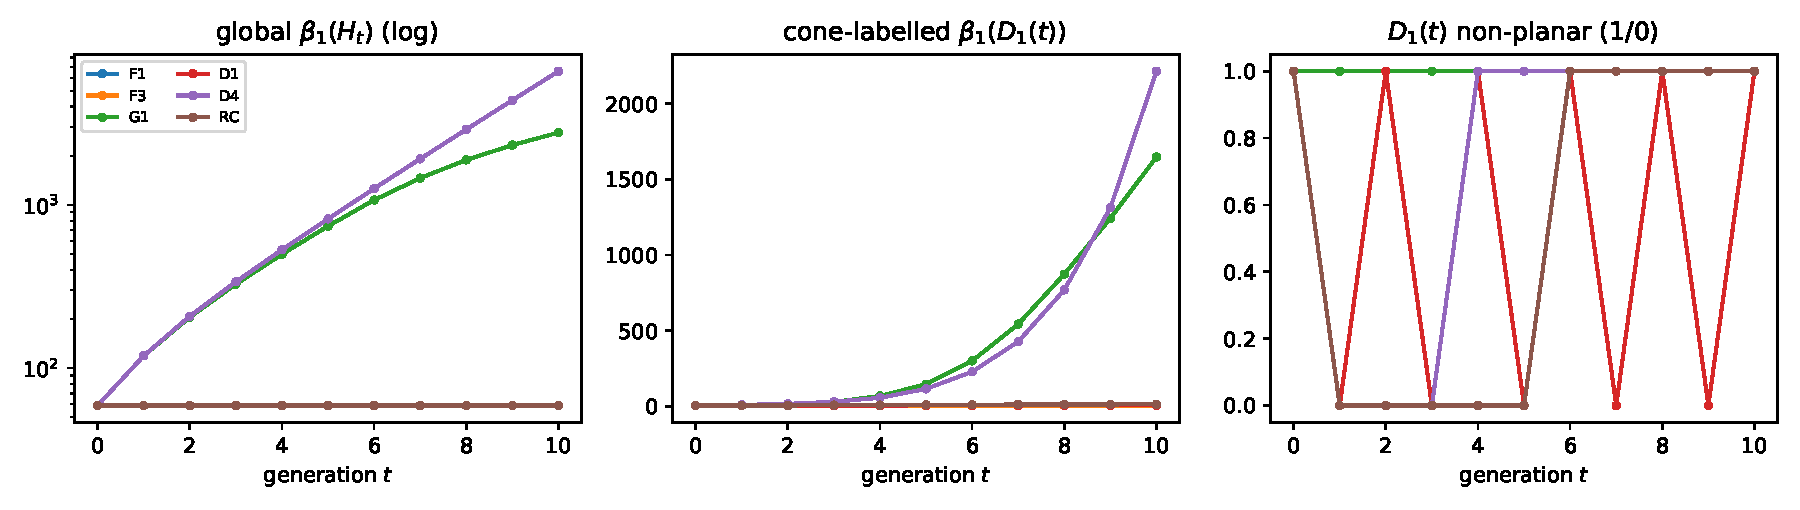
\includegraphics[width=\textwidth]{figs/fig_beta1.pdf}
\caption{Single $K_5$ on the 2D grid, canonical order. Left: global $\beta_1(H_t)$ (log axis). Middle: cone-labelled $\beta_1(D_1(t))$. Right: non-planarity of the cone-labelled $D_1(t)$; the oscillating curves are rules whose cone-labelled subgraph re-absorbs lattice edges.}\label{fig:beta1}
\end{figure*}

\section{Literature search protocol and log}\label{app:lit}
\paragraph{Protocol.} Searches were run on 16 November 2026. Sources: a general web search tool (English) and, for bibliographic databases, the public APIs of arXiv (Atom API) and INSPIRE-HEP; queries to the zbMATH Open API and to Semantic Scholar failed (HTTP 404/403 and 429) and MathSciNet and Scopus were not accessible. A reference is cited only if its title, authors and venue (or arXiv identifier) were confirmed from a retrieved record; items whose content could not be read are cited with a note. Inclusion criteria: work on (i) particles, defects or non-planar structures in Wolfram-model rewriting; (ii) causal invariance and confluence of hypergraph rewriting; (iii) topological or homological invariants of rewriting states; (iv) braid/ribbon particle models; (v) the graph-theoretic and curvature tools used here. A negative result means ``not found by these queries''.
\begin{table*}[t]\centering\scriptsize
\begin{tabular}{p{0.4cm}p{5.2cm}p{9.2cm}}
\toprule
\# & Query & Outcome\\
\midrule
1 & web: oligons, particles, topological defects, Wolfram model & Wolfram essays and technical introduction; Winter School 2021 $K_5$-in-tiling project (repository abstract); Gorard's tangle remarks. Cited.\\
2 & Gorard (2020b), full text, tangles & Read via HTML rendering: \S2.4 conditional heuristic on planarity-preserving rules, annihilation, charge analogy; Noether analogue deferred; ``oligon'' not used in that paper.\\
3 & web: causal invariance, confluence, critical pairs & Gorard 2020 (arXiv:2011.12174); Grossberndt notebook (experimental prover). Cited.\\
4 & arXiv API: ``Wolfram model'' with planar/defect/particle/topological & 2 records, all by Gorard on relativity/numerical GR; none on non-planar structures, defects or invariants.\\
5 & arXiv API: ``hypergraph rewriting'' with topological/homology/planarity/invariant & 3 records (Gorard); none relevant to (a)--(c) of our criteria.\\
6 & INSPIRE-HEP: ``hypergraph rewriting'' or ``Wolfram model'' in title/abstract & 8 records; closest: Arsiwalla--Gorard homotopy types (published Int.\ J.\ Theor.\ Phys.\ 63(4), 2024); none on defects, non-planarity or Betti numbers by title. Confirmed DOI of Gorard (2020b).\\
7 & INSPIRE-HEP: ``non-planar'' and ``graph rewriting'' in abstract & 0 records.\\
8 & zbMATH Open API, Semantic Scholar & Failed (404/403/429); no records.\\
9 & Lin--Lu--Yau; Bourne et al.; Wagner (1937); Ehrig et al.; Plump & Verified by web records (Ehrig book authors are Ehrig, Ehrig, Prange, Taentzer; Plump 2005 start page 280, end page unconfirmed; a second Plump title could not be verified and is not cited).\\
10 & Bilson-Thompson--Markopoulou--Smolin; Chester--Arsiwalla--Kauffman & Verified (Class.\ Quantum Grav.\ 24, 3975; arXiv:2501.03260).\\
11 & web: Betti numbers as conserved quantity in hypergraph rewriting & No source found.\\
12 & Patarroyo post; Summer School 2020 stable-defect project; technical-introduction page & Post exists, content not read; 2020 project not found; page listed by search but not fetchable (DNS failure) and not read.\\
\bottomrule
\end{tabular}
\caption{Literature search log (16 November 2026).}
\end{table*}
\noindent MathSciNet, zbMATH and Scopus were not searched, and no citation-chain search of the cited works was made.

\section{Guide to the archive}\label{app:guide}
Table~\ref{tab:guide} maps the computations of this paper to files of the archive (paths relative to the archive root) and to the scripts that produce them. \texttt{README.md} in the archive repeats the table together with the commands to regenerate every table and figure (\texttt{paper/generated}, \texttt{paper/figs}). Software versions are in Appendix~\ref{app:audit}; all random choices are seeded (global seed 20240601).
\begin{table*}[t]\centering\scriptsize
\begin{tabular}{>{\raggedright\arraybackslash}p{2.6cm}>{\raggedright\arraybackslash}p{2.1cm}>{\raggedright\arraybackslash}p{4.0cm}>{\raggedright\arraybackslash}p{3.4cm}}
\toprule
Item & In this paper & Archive files & Scripts\\
\midrule
Rule enumeration and counts & App.~\ref{app:audit}, Tab.~\ref{tab:enum} & \path{results/necessity/necessity_summary.csv} & \path{necessity_certificates.py}; \path{code/general_rules.py}\\
Certificates (Theorem~\ref{thm:dichotomy}) & Sec.~\ref{sec:class}, App.~\ref{app:audit} & \path{results/necessity/certificates.jsonl}; \path{results/necessity/verify_log.txt} & \path{necessity_certificates.py}; \path{verify_certificates.py}\\
Independent checks (\texttt{selftest}), counterexamples & App.~\ref{app:audit} & \path{results/selftest_log.txt}; \path{results/verify_independent_log.txt}; \path{results/counterexamples_log.txt} & \path{code/oligon_experiment.py}; \path{verify_independent.py}; \path{verify_counterexamples.py}\\
Classification on isolated $K_5$, $K_{3,3}$ & App.~\ref{app:exp}, Tab.~\ref{tab:class} & \path{results/classification/} & \path{classify_rules.py}\\
Joinability census (\texttt{census}) & App.~\ref{app:exp}, Tab.~\ref{tab:census} & \path{results/census/}; \path{results/census_2_4/} & \path{code/oligon_experiment.py}\\
Search beyond $\mathcal S$ & Sec.~\ref{sec:general}, Tab.~\ref{tab:general} & \path{results/general_1/}; \path{general_2k/}; \path{general_3/} & \path{general_signature_search.py}\\
Lattice runs, 126 joinable rules & Sec.~\ref{sec:exp}, Tab.~\ref{tab:joinable}, Fig.~\ref{fig:coll} & \path{results/rules_joinable.txt}; \path{results/rules_joinable_runs*/} & \path{run_all_joinable.sh}; \path{run_selected.py}; \path{analyze_joinable.py}\\
Lattice runs, selected rules & App.~\ref{app:exp} & \path{results/rules_selected.txt}; \path{results/runs*/} & \path{run_selected.py}; \path{analyze_results.py}\\
Wolfram-model rules & Sec.~\ref{sec:wolfram} & \path{results/wolfram_rules/} & \path{run_wolfram_rules.sh}; \path{wolfram_bridge_study.py}; \path{analyze_wolfram_rules.py}; \path{code/wolfram_bridge.py}\\
Planarity-preserving rules & Sec.~\ref{sec:planarity}, Tab.~\ref{tab:planarity} & \path{results/planarity/} & \path{planarity_preserving.py}\\
Non-injective check & Prop.~\ref{prop:noninj} & \path{results/noninjective_minor_check.txt} & \path{check_noninjective_minor.py}\\
Incidence-graph check & Sec.~\ref{sec:wolfram} & \path{results/incidence_check.txt} & \path{check_incidence_formula.py}\\
Tables and figures & all & \path{paper/generated/}; \path{paper/figs/} & \path{analyze_results.py}; \path{analyze_joinable.py}; \path{analyze_wolfram_rules.py}\\
\bottomrule
\end{tabular}
\caption{Where to find the experimental material (scripts are in \texttt{scripts/} unless a path is given).}\label{tab:guide}
\end{table*}

\bibliographystyle{plainnat}
\bibliography{references}
\end{document}
